\documentclass{report}
\usepackage[utf8]{inputenc}
\usepackage{amssymb}
\usepackage{amsmath}
\usepackage{graphicx}
\usepackage{mathpartir}
\usepackage[margin=1.5in]{geometry}
\usepackage{verbatim}
\usepackage{subfig}
\usepackage{wrapfig}
\usepackage{float}
\usepackage{bold-extra}
\usepackage{tikz}
\usepackage{palatino}
\usepackage{courier}
% \usepackage{textcomp} % Supports the Text Companion fonts which
% provide many text symbols (such as baht, bullet, copyright,
% musicalnote, onequarter, section, and yen) in the TS1 encoding.

\makeatletter
\newcommand*{\rom}[1]{\text{\footnotesize\expandafter\@slowromancap\romannumeral #1@.}}
\makeatother

\usepackage{listings}
\lstset{ %
  language=Haskell,                % the language of the code
  basicstyle=\ttfamily\footnotesize,           % the size of the fonts that are used for the code
%  numbers=left,                   % where to put the line-numbers
%  numberstyle=\footnotesize,          % the size of the fonts that are used for the line-numbers
%  stepnumber=2,                   % the step between two line-numbers. If it's 1, each line
%                                  % will be numbered
%  numbersep=5pt,                  % how far the line-numbers are from the code
  backgroundcolor=\color{white},      % choose the background color. You must add \usepackage{color}
  showspaces=false,               % show spaces adding particular underscores
  showstringspaces=false,         % underline spaces within strings
  showtabs=false,                 % show tabs within strings adding particular underscores
  frame=single,                   % adds a frame around the code
  tabsize=2,                      % sets default tabsize to 2 spaces
  captionpos=r,                   % sets the caption-position to bottom
  breaklines=true,                % sets automatic line breaking
  breakatwhitespace=false,        % sets if automatic breaks should only happen at whitespace
  title=\lstname,                   % show the filename of files included with \lstinputlisting;
                                  % also try caption instead of title
  numberstyle=\tiny\color{gray},        % line number style
  keywordstyle=\bfseries,          % keyword style
  commentstyle=\color{dkgreen},       % comment style
  stringstyle=\color{mauve},         % string literal style
  escapeinside={\%*}{*)},            % if you want to add a comment within your code
  morekeywords={*,...}               % if you want to add more keywords to the set
}

\newcommand\note[1]{\mbox{}\marginpar{\footnotesize\raggedright\hspace{0pt}\emph{#1}}}
\newcommand\hs[1]{\verb~#1~}
\newcommand\fn[1]{\mathrm{#1}}
\newcommand\ptr[1]{\fn{#1.ptr}}
\newcommand\appfn{@}
\newcommand\app[2]{#1 \, \appfn \, #2}
\newcommand\ex[1]{\exists \, #1 \, . \,}
\newcommand\nexxx[3]{\nexists \, #1 , #2 , #3 . \,}
\newcommand\fa[1]{\forall \, #1 . \,}
\newcommand\faa[2]{\forall \, #1 , #2 . \,}
\newcommand\faaa[3]{\forall \, #1 , #2 , #3 . \,}
\newcommand\faaaaaa[6]{\forall \, #1 , #2 , #3 \, #4 , #5 , #6 . \,}

\newcommand\tofix[1]{#1_{\mathrm{tofix}}}
\newcommand\unfix[1]{#1_{\mathrm{unfix}}}

\newcommand{\xsys}[2]{#1 \, xs \, #2 & = #1 \, ys #2}
\newcommand{\desca}[1]{  & \hspace{44.5mm}                            \{ \mathrm{#1} \}}
\newcommand{\descra}[1]{ & \hspace{35mm} \Rightarrow     \hspace{4mm} \{ \mathrm{#1} \}}
\newcommand{\descla}[1]{ & \hspace{35mm} \Leftarrow      \hspace{4mm} \{ \mathrm{#1} \}}
\newcommand{\desclra}[1]{& \hspace{35mm} \Leftrightarrow \hspace{4mm} \{ \mathrm{#1} \}}

\newcommand\lub[1]{\sqcup_{#1}}
\newcommand\defof[1]{definition \, of \, #1}

\newcommand\w[0]{\,\,}
\newcommand\eq[0]{ = }

\newcommand{\defBNF}[4] {\text{#1}\quad&#2&::=&\;#3&\text{#4}}
\newcommand{\defaltBNF}[2] {&&|&\;#1&\text{#2}}

\begin{document}

\noindent
\chapter{Haskell to First Order Logic}

To enable automated theorem provers to do equational reasoning of
Haskell programs a translation to first order logic is needed. It is
here referred to as a translation, but it could also be regarded as a
compilation. The idea is to use constants and functions in first order
logic to correspond to constructors and functions, and arguments to
functions need to be universally quantified. We shall try to do a
na\"{\i}ve attempt of a translation with this ideas and see how far it
takes us.

\section{Na\"{\i}ve Translation}

We will use a data type of binary trees with an element at every
branch, and consider some examples of functions defined on it. This
is the Haskell definition of the data type we will be using:

\begin{code}
data Tree a = Fork (Tree a) a (Tree a) | Leaf
\end{code}

\noindent
With the idea above, occurrences of the \hs{Fork} constructor in the
source code should be translated to a logic function $\fn{fork}$, and
similarly a constant for \hs{Leaf}. How should we then translate the
\hs{singleton} function, defined below?

\begin{code}
singleton :: a -> Tree a
singleton x = Fork Leaf x Leaf
\end{code}

\noindent
Following our intuition we make an universal quantification for
\hs{x}, and a new logic function for \hs{singleton}. The result
is this axiom:
\begin{equation*}
\fa{x} \fn{singleton}(x) = \fn{fork}(\fn{leaf},x,\fn{leaf})
\end{equation*}

\noindent
So far so good, but what if someone wants to prove that \hs{singleton x}
is a \hs{Leaf}? With only this axiom in the theory, it would be
possible: there are models with only one element where \hs{Leaf} is
equal to \hs{Fork}. Indeed, we will need to add axioms that values
created from the different constructors are unequal. We will call
those disjoint constructor axioms, and for the \hs{Tree} data type, we
get this axiom:
\begin{equation*}
\faaa{l}{x}{r} \fn{leaf} \neq \fn{fork}(l,x,r)
\end{equation*}

Constructors should also be injective to get regular models, and
adding such axioms are straightforward. Since only \hs{Fork} has
arguments, this injectivity axiom is needed:
\begin{equation*}
\faaaaaa{l_0}{l_1}{x_0}{x_1}{r_0}{r_1} \fn{fork}(l_0,x_0,r_0) \eq
\fn{fork}(l_1,x_1,r_1) \rightarrow l_0 \eq l_1 \wedge x_0 \eq x_1 \wedge r_0 \eq r_1
\end{equation*}

For the \hs{mirror} function, which recursively mirrors the left sub
tree with the right and vice-versa, we follow our intuition to
translate the pattern matching and get these two axioms\footnote
{Axioms are enumerated by Roman numerals to tell them apart.}:

\begin{code}
mirror :: Tree a -> Tree a
mirror (Fork l x r) = Fork (mirror r) x (mirror l)
mirror Leaf         = Leaf
\end{code}
\begin{align*}
\rom{1} && \faaa{l}{x}{r} & \fn{mirror}(\fn{fork}(l,x,r)) \eq \fn{fork}(\fn{mirror}(r),x,\fn{mirror}(l)) \\
\rom{2} &&                & \fn{mirror}(\fn{leaf}) \eq \fn{leaf}
\end{align*}

\noindent
A problem with this translation is that there are no axioms for other
arguments of $\fn{mirror}$ than leafs and forks, and we have models that
include other values than leafs and forks. Another problem is
encountered for \hs{singleton}'s left inverse, \hs{top}, code below,
which returns the top element of a \hs{Tree}. This is a partial
function since it has no pattern for the \hs{Leaf} constructor.

\begin{code}
top :: Tree a -> a
top (Fork l x r) = x
\end{code}

The translation must capture the pattern match failure that results
from trying to evaluate top applied to a leaf. We conclude that
this na\"{\i}ve translation does not take us further, but we shall see
in the next section how to fix this.

\section{Bottom and Pattern Matching}

In domain theory there is a concept of bottom, denoted $\bot$. It is
used for the least defined value: pattern match failures, use of
\hs{error} and \hs{undefined} in the source code, but also for
non-terminating programs. For \hs{top} the idea is to add an axiom so
that $\fn{top}$ of anything that is not a \hs{Fork} is bottom. This is
an example of such an axiomatization:

\begin{align*}
\rom{1} \qquad & \faaa{l}{x}{r} \fn{top}(\fn{fork}(l,x,r)) \eq x \\
\rom{2} \qquad & \fa{t}         (\nexxx{l}{x}{r} \fn{fork}(l,x,r)) \eq t) \rightarrow \fn{top}(t) \eq \bot
\end{align*}

Most theorem provers would as a preprocessing step \note{\qquad \qquad citation
  needed}skolemize the existential quantification in the second
axiom. A new unary function would be introduced for $l$, $x$ and $r$,
depending on $t$, an arbitrary choice of names are $\fn{top}$ appended
to the original variable. The axiom then looks like
this\footnote{Lambda functions bind as far to the right as possible,
  and this thesis uses the same convention for quantifiers.}:
\begin{align*}
\rom{2}' \qquad & \fa{t} \fn{fork}(\fn{topl}(t),\fn{topx}(t),\fn{topr}(t))) \neq t \rightarrow \fn{top}(t) \eq \bot
\end{align*}

For another function, like \hs{mirror} above, one of the skolemized
functions could be called $\fn{mirrorl}$. Since axioms of injective
constructors are also added, a theorem prover could, in some steps,
conclude that $\faaa{l}{x}{r} \fn{mirrorl}(\fn{fork}(l,x,r)) \eq
\fn{topl}(\fn{fork}(l,x,r)) \eq l$. But what happens if we introduce
such skolemized ``selector'' functions for every constructor manually?
For the \hs{Fork} constructor call them $\fn{fork_0}$, $\fn{fork_1}$
and $\fn{fork_2}$, and their axioms are:
\begin{align*}
\rom{1} \qquad \faaa{l}{x}{r} \fn{fork_{0}}(\fn{fork}(l,x,r)) & \eq l \\
\rom{2} \qquad \faaa{l}{x}{r} \fn{fork_{1}}(\fn{fork}(l,x,r)) & \eq x \\
\rom{3} \qquad \faaa{l}{x}{r} \fn{fork_{2}}(\fn{fork}(l,x,r)) & \eq r
\end{align*}

\noindent
The translation of \hs{top} with these selector functions is:
\begin{align*}
\rom{1} \qquad & \faaa{l}{x}{r} \fn{top}(\fn{fork}(l,x,r)) \eq x \\
\rom{2} \qquad & \fa{t}         (\fn{fork}(\fn{fork_0}(t),\fn{fork_1}(t),\fn{fork_2}(t))) \neq t) \rightarrow \fn{top}(t) \eq \bot
\end{align*}

\noindent
Another nice side effect of writing in this skolemized selector style
is that implies injective constructors. Assume we have
$\fn{fork}(l_0,x_0,r_0)=\fn{fork}(l_1,x_1,r_1)$ then the first
projection, $\fn{fork_0}$, gives us that $l_0=l_1$. Analogously, and
the second and the third give $x_0=x_1$ and $r_0=r_1$,
respectively. Thus selector axioms are added in place of of
injectivity axioms.

With the bottom constant in the theory, the axioms disjointedness are
effected by this. It can be seen as an implicit constructor for every
data type. For the \hs{Tree} data type the axioms are:

\begin{align*}
\rom{1} \qquad & \faaa{l}{x}{r} \fn{fork}(l,x,r) \neq \fn{leaf} \\
\rom{2} \qquad & \faaa{l}{x}{r} \fn{fork}(l,x,r) \neq \bot      \\
\rom{3} \qquad & \bot \neq \fn{leaf}
\end{align*}

Now we have a good idea how to translate pattern matching, but
in Haskell we can pattern match almost everywhere! How would we
proceed to translate a function like this, taken from the
implementation of \hs{scanr} from the \hs{Prelude}?

\begin{code}
scanr             :: (a -> b -> b) -> b -> [a] -> [b]
scanr f q0 []     =  [q0]
scanr f q0 (x:xs) =  f x q : qs
                     where qs = scanr f q0 xs
                           q = case qs of
                                 q : _ -> q
\end{code}

\noindent
There is both pattern matching on the direct arguments, but also
pattern matching in a case statements in the where function
\hs{q}. There can also be pattern matching in lambdas. To help with
these difficulties, we define an intermediate language in the next
section.

\section{The Intermediate Language}

To address the difficulties of pattern matching elsewhere than the
arguments of a function, a small intermediate language was designed
that can only do pattern matching at a very controlled location: in a
case statement that is the entire body of a function, and all arms are
just simple expressions consisting of function and constructor
applications and variables. Haskell is translated to this, and pattern
matching at other locations is translated to this in a new top level
definition. Functions definined in let and where are raised to the top
level, with the necessary variables in scope as additional
arguments. The same is done for sections and lambda functions. The BNF
for the language is this:

\begin{equation*}
\begin{aligned}
\text{Variables} \quad & x \\
\text{Functions} \quad & f \\
\text{Constructors} \quad & C \\
\text{Type variables} \quad & \tau \\
\text{Type constructors} \quad & T \\
\defBNF{Declarations}{decl}{ f \; \overline{x} \; \hs{=} \; body}{function declaration} \\
    \defaltBNF{f \; :: \; t}{type signature} \\
    \defaltBNF{\hs{data} \; T \; \overline{\tau} \; \hs{=} \; \overline{C \; \overline{t}}}{data type declaration} \\
\defBNF{Function body}{body}{\hs{case} \; e \; \hs{of} \; \overline{alt}}{case body} \\
    \defaltBNF{e}{expression body} \\
\defBNF{Expressions}{e}{x}{variable} \\
    \defaltBNF{f \; \overline{e}}{function application} \\
    \defaltBNF{C \; \overline{e}}{constructor application} \\
\defBNF{Alternative}{alt}{pat \rightarrow e}{branch without guard} \\
    \defaltBNF{pat \; \hs{|} \; e \rightarrow e}{branch with guard} \\
\defBNF{Pattern}{p}{x}{pattern variable} \\
    \defaltBNF{C \; \overline{p}}{constructor pattern} \\
\defBNF{Types}{t}{\tau}{type variable} \\
    \defaltBNF{t \; \rightarrow \; t}{function type} \\
    \defaltBNF{T \; \overline{\tau}}{type constructor application} \\
\defBNF{Programs}{prog}{\overline{decl}}{} \\
\end{aligned}
\end{equation*}

This language is a strict subset of Haskell. Repeated entities are
notated with an $\overline{\text{overline}}$.  Data declarations are
added for disjointedness and selector axioms, and type signatures are
just skipped in the translation, but the proof techniques introduced
later use this information.

A function is just a function name with a number of variables, and
then a function body, which is either an expression of variables,
functions and constructors, or a case statements with an expression
scrutinee. Branches consists of a pattern, possibly with nested uses
of constructors, and an optional guard, and in the arm is an
expression.

Now we need to distinguish between two translations: the intermediate
translation from Haskell to the intermediate language, and the logic
translation from this language to first order logic.

\section{The Intermediate Translation}

After this section, we will only concentrate on the logic translation.

\paragraph{Argument pattern matching} A function that does pattern matching will be translated to one that
takes in unmatched arguments and with a case in the body. The
\hs{mirror} function above is thus translated to this:

\begin{code}
mirror :: Tree a -> Tree a
mirror t = case t of
   Fork l x r -> Fork (mirror r) x (mirror l)
   Leaf       -> Leaf
\end{code}

\noindent
If you do pattern matching on several arguments, the scrutinee in the
case will be a tuple of all the arguments.

\paragraph{Local definitions} Where-clauses and let-expressions are
raised to the top level, with all necessary variables as
arguments. This example of an accumulator definition of multiplication
of Peano natural numbers needs such a rewrite:

\begin{code}
(*) :: Nat -> Nat -> Nat
x * y = go Zero x
  where
    go acc Zero    = acc
    go acc (Suc n) = go (acc + y) n
\end{code}

\noindent
The \hs{go} function has the \hs{y} in scope but not as argument so it
is appended to the arguments to the top level lifted version of \hs{go}:

\begin{code}
go acc Zero    y = acc
go acc (Suc n) y = go (acc + y) n y

x * y = go Zero x y
\end{code}

\noindent
Finally \hs{go} is translated using a case expression:

\begin{code}
go acc x y = case x of
     Zero  -> acc
     Suc n -> go (acc + y) n y
\end{code}

A similar translation is done for let expressions.

\paragraph{Lambda functions} These are translated to top level
definitions. Take this example of defining \hs{fmap} in terms of the
functions from the \hs{Monad} type class:

\begin{code}
fmap' :: Monad m => (a -> b) -> m a -> m b
fmap' f m = m >>= \x -> return (f x)
\end{code}

\noindent
In the lambda, \hs{f} is a free variable so it becomes an argument to
the new top level function called \hs{lambda} below:

\begin{code}
lambda f x = return (f x)

fmap' :: Monad m => (a -> b) -> m a -> m b
fmap' f m = m >>= lambda f
\end{code}

A similar translation is done for sections.

\section{Pattern Matching Revisited}

\paragraph{Overlapping patterns} First of all, overlapping patterns need to be removed, otherwise we
easily get an inconsistent theory, consider

\begin{code}
overlap :: Bool -> Bool
overlap b = case b of
              True -> True
              True -> False
\end{code}

Certainly, this cannot be translated to:
\begin{align*}
\rom{1} \qquad & \fn{overlap}(\fn{true}) = \fn{true} \\
\rom{2} \qquad & \fn{overlap}(\fn{true}) = \fn{false} \\
\rom{3} \qquad & \fa{b} b \neq \fn{true} \rightarrow \fn{overlap}(b) = \bot
\end{align*}

Starting from the immediate truth $\fn{overlap}(\fn{true}) =
\fn{overlap}(\fn{true})$, transitivity of the equalities in the axioms
$\romnodot{1}$ and $\romnodot{2}$ gives the equality $\fn{true} =
\fn{false}$. This together with the axiom from disjoint constructors,
$\fn{true} \neq \fn{false}$, gives a contradiction.

In Haskell, pattern matching is done from top to bottom of the
definition, making the second match of \hs{True} to never occur. Thus,
the translation to FOL also removes all subsequent patterns that are
instances of any pattern above.

\paragraph{Nested patterns and bottoms} The translation also handles
patterns in more than one depth. At every location in a pattern where
a constructor is matched against, a pattern with bottom at that spot
is also added, defined to bottom. This Haskell function \hs{even}
determines if a list is of even length:

\begin{code}
even :: List a -> Bool
even (Cons x (Cons y ys)) = even ys
even (Cons x xs)          = False
even Nil                  = True
\end{code}

\noindent
For the sake of readability it is not presented with a case
expression, though this is what the intermediate translation would
transform it to. Furthermore the constructors \hs{Cons} and \hs{Nil}
are used since the projections $\fn{:_0}$ and $\fn{:_1}$ for the
normal cons are hard to read.

For each matched constructor, we need to add a new match to bottom,
which evaluates to bottom. Unnecessary bottoms can be carelessly added
since overlapping patterns are removed \emph{afterwards}. Furthermore,
a wild pattern is added at the end that goes to bottom in case there
are other constructors for the data type not mentioned in the
patterns.

No type information is needed to do this: it is merely an
inspection. Could the bottoms be seen in this Haskell definition it
would be this after the insertion of bottoms:

\begin{code}[mathescape]
even :: List a -> Bool
even (Cons x (Cons y ys)) = even ys
even (Cons x $\bot$)            = $\bot$
even $\bot$                     = $\bot$
even (Cons x xs)          = False
even Nil                  = True
even _                    = $\bot$
\end{code}

Haskell's behavior of matching patterns from top to bottom is
justified with implications ensuring the \emph{upward agreement}. The
axioms for this definitions are:
\newcommand\uncons[1]{\cons{\fn{cons_0}(#1)}{\fn{cons_1}(#1)}}
\newcommand\even[1]{\fn{even}(#1)}
\newcommand\cons[2]{\fn{cons}(#1,#2)}
\begin{align*}
\rom{1} && \faaa{x}{y}{ys} & \even{\cons{x}{\cons{y}{ys}}} = \even{ys} \\
\rom{2} && \fa{x}          & \even{\cons{x}{\bot}}         = \bot      \\
\rom{3} &&                 & \even{\bot} = \bot \\
\rom{4} && \faa{x}{xs}     & xs \neq \uncons{xs} \wedge xs \neq \bot \rightarrow \even{\cons{x}{xs}} = \fn{false}  \\
\rom{5} &&                 & \even{\fn{nil}} = \fn{true} \\
\rom{6} && \fa{xs}         & xs \neq \fn{nil} \wedge
                             xs \neq \uncons{xs} \wedge
                             xs \neq \bot \rightarrow \even{xs} = \bot
\end{align*}

Some room for improvement can be seen: the inserted
\hs{even }$\bot$\hs{ = }$\bot$ case is redundant as it is implied by
the wild pattern to $\bot$. The upward agreement implications can
readily be seen, an example is
$xs \neq \uncons{xs} \wedge xs \neq \bot$ in axiom $\romnodot{3}$.

\section{Functions as Arguments}

In Haskell, functions readily take other functions as arguments, and
functions can also be partially applied. To get the same behavior in
logic, each function gets a \emph{function pointer}, and a new binary
function is added to the language, written infix with $\appfn$.  For
instance if there is a binary function \hs{plus} then a constant
called $\fn{plus.ptr}$ is added to the theory and this axiom:

\begin{equation*}
\faa{x}{y}  \app{(\app{\fn{plus.ptr}}{x})}{y} = \fn{plus}(x,y)
\end{equation*}

When a function is only partially applied, or a function argument is
applied, $\appfn$ is used. Consider this Prelude function \hs{iterate}:

\begin{code}
iterate :: (a -> a) -> a -> [a]
iterate f x = x : iterate f (f x)
\end{code}

It is translated with $\appfn$ in the following way, with the cons
constructor \hs{:} written infix:

\begin{equation*}
\forall \, f \, x \, . \, \fn{iterate}(f,x) = x : \fn{iterate}(f,\app{f}{x})
\end{equation*}

Should a function not get all its arguments, appropriate use of $\, @ \, $ is
added, as in this function which increments all elements of the list
by one using \hs{map}:

\begin{code}
incr = map (plus one)
\end{code}

As \hs{incr} is written $\eta$-reduced, \hs{map} is
only partially applied, this is the translated axiom:

\begin{equation*}
\fn{incr} = \app{\fn{map.ptr}}{(\app{\fn{plus.ptr}}{\fn{one}})}
\end{equation*}

If \hs{incr} is applied to an argument $xs$, then \hs{incr} is applied
to more arguments than it takes, so we add $\appfn$ so the
corresponding formula becomes $\app{\fn{incr}}{xs}$, and by equational
substitution from the definition of $\fn{incr}$ we get
$\app{(\app{\fn{map.ptr}}{(\app{\fn{plus.ptr}}{\fn{one}})})}{xs}$ and
the axiom of $\fn{map.ptr}$ then equals this to
$\fn{map}(\app{\fn{plus.ptr}}{\fn{one}},xs)$.

\paragraph{Doing the impossible}
While it is not possible to quantify over functions in first order
logic, translating Haskell this way allows universal quantification of
functions.  It provides a way to reason syntactically about partially
applied functions. On the model side, $\appfn$ gives a way to
interpret functions and universally quantify over them. If the
function has a pointer defined, it just constrains app on that pointer
to do the same as the function.

\section{Guards}

Guards are treated much like pattern matching. If a
guard expression evaluates to \hs{True}, that branch is picked. The
expression could also evaluate to $\bot$, and then the result should
be $\bot$. Let us consider the \hs{filter} function:

\begin{code}
filter :: (a -> Bool) -> List a -> List a
filter p (Cons x xs) | p x = Cons x (filter p xs)
filter p (Cons x xs)       = filter p xs
filter p Nil               = Nil
\end{code}


To translation this to logic it is needed to ensure that if \hs{p x}
evaluates to $\bot$, then so should the function. The axioms look
like this:
\newcommand\filter[2]{\fn{filter}(#1,#2)}
\begin{align*}
\rom{1} && \faaa{p}{x}{xs} & (\app{p}{x}) = \fn{true}                                  \rightarrow \filter{p}{\cons{x}{\cons{y}{ys}}} = \cons{x}{\filter{p}{xs}} \\
\rom{2} && \faaa{p}{x}{xs} & (\app{p}{x}) = \bot                                       \rightarrow \filter{p}{\cons{x}{\cons{y}{ys}}} = \bot \\
\rom{3} && \faaa{p}{x}{xs} & (\app{p}{x}) \neq \fn{true} \wedge (\app{p}{x}) \neq \bot \rightarrow \filter{p}{\cons{x}{\cons{y}{ys}}} = \filter{p}{xs} \\
\rom{4} &&                 & \filter{p}{\fn{nil}} = \fn{nil} \\
\rom{5} && \fa{xs}         & xs \neq \fn{nil} \wedge xs \neq \uncons{xs} \rightarrow \filter{p}{xs} = \bot
\end{align*}

\section{Summary}

The translation of different Haskell concepts is summarized in
Table~\ref{tab:transtable}.

\begin{table}[h]
  \centering
  \begin{tabular}{|l|l|}
    \hline
    Haskell                    & First Order Logic \\
    \hline
    function                   & function or constant \\
    constructor                & function or constant \\
    data type                  & disjoint constructors and selector axioms \\
    pattern matching           & overlap removal, bottoms insertion, upward agreement \\
    guards                     & equality to true and bottom and upward agreement \\
    partial application        & $\appfn$ on pointer constant \\
    partially applied function & pointer constant and $\appfn$ rule \\
    sections, lambdas, let     & new functions with variables in scope as arguments \\
    \hline
  \end{tabular}
  \caption{Translation of different Haskell constructs
    \label{tab:transtable}
  }
\end{table}

%Equational reasaoning is traditional in proving corrected of Haskell
%programs, but it assumes that a simple denotational semantics exists,
%and there is not even a formal semantics for the language
%\cite{chasingbot}.
%

% Remove unnecessary definitions for a given proof


%% Domain theory

\section{Domain Theory}
\label{sec:domaintheory}

This section is stand alone, and could be skipped especially if you
already know the basics of Domain Theory: comp\-lete partial orders,
monotonicity and continuity.
It explains these concepts and discusses how it can be
used to verify the translation, furthermore it is used as a reference
in the future sections that rely on concepts from domain theory.
%The section explains these concepts and acts as a reference in future
%sections that rely on concepts from domain theory.

The values of every data type are ordered on how much ``information''
they contain. The least element bottom, denoted $\bot$, contains least
information. It corresponds to all kinds of crashes in Haskell; use of
\hs{undefined}, non-termination or non exhausite pattern matches.
Different constructors hold different information, so they are not
related by the ordering; this is a partial order, a relation that is
reflexive, transitive and antisymmetric. The ordering is usually
written $\sqsubseteq$ sometimes with a subscript indicating the type.

\begin{wrapfigure}{O}{0.4\textwidth} %\begin{figure}
\vspace{-7pt}
\centering \begin{tikzpicture}[
    level distance=-1.5cm,
    growth parent anchor=north,
    sibling distance=3cm
]
\node {$\bot$}
    child {
        node {$\hs{True}$}
    }
    child {
        node {$\hs{False}$}
    };
\end{tikzpicture}


%\end{document}
\vspace{-7pt}
\caption{
    The order of Bool values.
    \label{fig:boolcpo}
}
\end{wrapfigure}
For the \hs{Bool} data type the partial order can be drawn as a Hasse
Diagram and this can be shown in Figure \ref{fig:boolcpo}.  From the
picture it is understood that $\bot$ is the least element, and the
line from it to \hs{False} means that $\bot \sqsubseteq \hs{False}$,
since $\bot$ is below $\hs{False}$. Correspondingly for $\hs{True}$,
the diagram tells us that $\bot \sqsubseteq \hs{True}$. It can also
been seen that $\hs{True} \nsqsubseteq \hs{False}$; they are unrelated
since there is no line between them.

%\begin{figure}[h]
%\centering
%\begin{tikzpicture}[
    level distance=-1.5cm,
    growth parent anchor=north,
    sibling distance=3cm
]
\node {$\bot$}
    child {
        node {$\hs{True}$}
    }
    child {
        node {$\hs{False}$}
    };
\end{tikzpicture}


%\end{document}
%\caption{The partial order for \texttt{Bool} as a Hasse Diagram
%  \label{fig:boolcpo}
%}
%\end{figure}

%\begin{figure}[h]
%  \centering
%  \subfloat[\texttt{Bool}]{\label{fig:boolcpo}\begin{tikzpicture}[
    level distance=-1.5cm,
    growth parent anchor=north,
    sibling distance=3cm
]
\node {$\bot$}
    child {
        node {$\hs{True}$}
    }
    child {
        node {$\hs{False}$}
    };
\end{tikzpicture}


%\end{document}}
%  \hspace{20pt}
%  \subfloat[\texttt{(Bool,Bool)}]{\label{fig:boolboolcpo}%\documentclass[10pt]{article}
\newcommand{\myGlobalTransformation}[2]
{
    \pgftransformreset;
    \pgftransformcm{1.6}{0}{0.65}{0.5}{\pgfpoint{#1cm}{#2cm}}
}

\newcommand\tru{\hs{T}}
\newcommand\fal{\hs{F}}

\newcommand\ddraw[2]{
        \draw[-,line width=3pt,draw=white] (#1) -- (#2);
        \draw (#1) -- (#2);
}

%\begin{document}
%\pagestyle{empty}

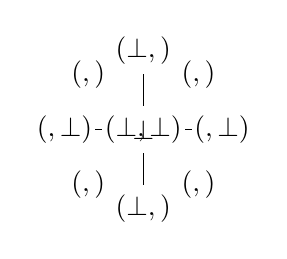
\begin{tikzpicture}

    \begin{scope}
        \myGlobalTransformation{0}{-0.4};
        \node (bottom) at (0,0) {$\bot$};

        \myGlobalTransformation{0}{0.9};
        \node (botbot) at (0,0) {$(\bot,\bot)$};

        \myGlobalTransformation{0}{3};
        \node (trubot) at (-1,0) {$(\tru,\bot)$};
        \node (bottru) at (0,1)  {$(\bot,\tru)$};
        \node (falbot) at (1,0)  {$(\fal,\bot)$};
        \node (botfal) at (0,-1) {$(\bot,\fal)$};

        \myGlobalTransformation{0}{5.5};
        \node (trutru) at (-0.7, 0.7) {$(\tru,\tru)$};
        \node (faltru) at ( 0.7, 0.7) {$(\fal,\tru)$};
        \node (falfal) at ( 0.7,-0.7) {$(\fal,\fal)$};
        \node (trufal) at (-0.7,-0.7) {$(\tru,\fal)$};

        \draw (bottom) -- (botbot);

        \draw (botbot) -- (trubot);
        \draw (botbot) -- (bottru);
        \draw (botbot) -- (falbot);
        \draw (botbot) -- (botfal);

        \ddraw{trubot}{trutru};
        \ddraw{bottru}{trutru};
        \ddraw{falbot}{faltru};
        \ddraw{bottru}{faltru};
        \ddraw{trubot}{trufal};
        \ddraw{botfal}{trufal};
        \ddraw{botfal}{falfal};
        \ddraw{falbot}{falfal};

    \end{scope}

\end{tikzpicture}

%\end{document}}
%  \caption{Two partial orders as Hasse Diagrams}
%  \label{fig:pos}
%\end{figure}

\begin{wrapfigure}[25]{r}{0.4\textwidth} %\begin{figure}\begin{figure}[h!]
\begin{center}
\vspace{-30pt}
%\documentclass[10pt]{article}
\newcommand{\myGlobalTransformation}[2]
{
    \pgftransformreset;
    \pgftransformcm{1.6}{0}{0.65}{0.5}{\pgfpoint{#1cm}{#2cm}}
}

\newcommand\tru{\hs{T}}
\newcommand\fal{\hs{F}}

\newcommand\ddraw[2]{
        \draw[-,line width=3pt,draw=white] (#1) -- (#2);
        \draw (#1) -- (#2);
}

%\begin{document}
%\pagestyle{empty}

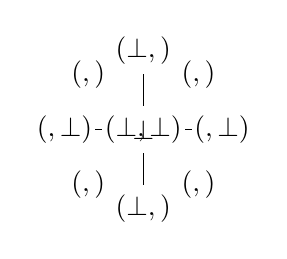
\begin{tikzpicture}

    \begin{scope}
        \myGlobalTransformation{0}{-0.4};
        \node (bottom) at (0,0) {$\bot$};

        \myGlobalTransformation{0}{0.9};
        \node (botbot) at (0,0) {$(\bot,\bot)$};

        \myGlobalTransformation{0}{3};
        \node (trubot) at (-1,0) {$(\tru,\bot)$};
        \node (bottru) at (0,1)  {$(\bot,\tru)$};
        \node (falbot) at (1,0)  {$(\fal,\bot)$};
        \node (botfal) at (0,-1) {$(\bot,\fal)$};

        \myGlobalTransformation{0}{5.5};
        \node (trutru) at (-0.7, 0.7) {$(\tru,\tru)$};
        \node (faltru) at ( 0.7, 0.7) {$(\fal,\tru)$};
        \node (falfal) at ( 0.7,-0.7) {$(\fal,\fal)$};
        \node (trufal) at (-0.7,-0.7) {$(\tru,\fal)$};

        \draw (bottom) -- (botbot);

        \draw (botbot) -- (trubot);
        \draw (botbot) -- (bottru);
        \draw (botbot) -- (falbot);
        \draw (botbot) -- (botfal);

        \ddraw{trubot}{trutru};
        \ddraw{bottru}{trutru};
        \ddraw{falbot}{faltru};
        \ddraw{bottru}{faltru};
        \ddraw{trubot}{trufal};
        \ddraw{botfal}{trufal};
        \ddraw{botfal}{falfal};
        \ddraw{falbot}{falfal};

    \end{scope}

\end{tikzpicture}

%\end{document}
\caption{
    \texttt{(Bool,Bool)} partial order.
    \label{fig:boolboolcpo}
}
\end{center}
\end{wrapfigure} %\end{figure}
For tuples and other constructors that take other data types as
parameters, the ordering is:
\begin{equation*}
\hstup{x_0}{y_0} \sqsubseteq_{(a,b)} \hstup{x_1}{y_1} \text{\quad iff \quad}
x_0 \sqsubseteq_a x_1 \text{\w and \w} y_0 \sqsubseteq_b y_1
\end{equation*}

The Hasse Diagram for the \hs{(Bool,Bool)} values can be seen in
Figure \ref{fig:boolboolcpo}. Here \hs{True} is abbreviated for \hs{T}
and similarly for \hs{False}. It is not flat as the one for \hs{Bool};
it can be seen as three dimensional. On the lowest layer the only
value is $\bot$, on the next layer $\hstup{\bot}{\bot}$. Above that
the tuples with one $\bot$, and finally the total values at the
top.

\vspace{55pt}

\subsection{Monotonicity}
 An important property all safe Haskell functions have is that they are
monotone with respect to this ordering.

\paragraph{Definition} A function $f$ is \emph{monotone} iff

\begin{equation*}
\faa{x}{y} \quad x \sqsubseteq y \quad \Rightarrow \quad f(x) \sqsubseteq f(y).
\end{equation*}

This can be understood in many ways. One way to see it is if you have
two inputs to a function, one containing \emph{less} information that
the other, i.e. more bottoms, it is impossible to return \emph{more}
information from the input with less information.

\newpage

One simple example of a consequence of this is the impossibility to
make a function \hs{isBottom :: a -> Bool}, returning \hs{True} if the
argument is bottom, and \hs{False} otherwise:

\note{rewrite with code}
\begin{align*}
& \hs{isBottom} \w :: \hs{a} \rightarrow \hs{Bool} \\
& \hs{isBottom} \w \bot = \hs{True} \\
& \hs{isBottom} \w x \, = \hs{False}, \qquad x \neq \bot
\end{align*}

\noindent
Since $\bot \sqsubseteq x$ for any $x$, then by monotonicity we must
necessarily have
$$\hs{isBottom} \w \bot \sqsubseteq \hs{isBottom} \w x.$$
Take any non-bottom $x$, and this equation gives
$\hs{True} \sqsubseteq \hs{False}$, which is false. Hence
\hs{isBottom} is not monotone.

\subsection{Continuity}
Another domain theoretic property that Haskell functions have is that
they are continuous. This is a property that gives us insight in how
functions behave on infinite input.  To describe this, we need to
consider the partial order of a data type with infinite values. The
prime candidate \hs{data Nat = Zero | Succ Nat} is used and Hasse
Diagram can be seen in Figure \ref{fig:natcpo}.

\begin{figure}[h]
\centering
\usetikzlibrary{positioning,shadows,arrows}

\def\adots{\mathinner{\mkern2mu\raise\hbox{.}
\mkern2mu\raise4\hbox{.}\mkern1mu
\raise8\vbox{\kern7\hbox{.}}\mkern1mu}}


%\begin{tikzpicture}[scale=10]
%
%  \node (bottom)                          {$\bot$};
%  \node (zero)        [above=of bottom]   {$Zero$};
%  \node (suc bot)     [right=of zero]     {$Suc \, \bot$};
%  \node (suc zero)    [above=of suc bot]  {$Suc \, Zero$};
%  \node (suc suc bot) [right=of suc zero] {$Suc \, (Suc \, \bot)$};
%
%  \draw [-] (bottom) -- (zero);
%  \draw [-] (bottom) -- (suc bot);
%  \draw [-] (suc bot) -- (suc zero);
%  \draw [-] (suc bot) -- (suc suc bot);
%
%\end{tikzpicture}
%
\begin{tikzpicture}[grow'=up,sibling distance=2cm]
\node {$\bot$}
    child {
        node {$\hs{Zero}$}
    }
    child {
        node {$\hs{Succ} \, \bot$}
        child {
            node {$\hs{Succ} \, \hs{Zero}$}
        }
        child {
            node {$\hs{Succ} \, (\hs{Succ} \, \bot)$}
            child {
                node {$\hs{Succ} \, (\hs{Succ} \, \hs{Zero})$}
            }
            child {
              node {$ ^{ ^{\adots}}$}
              child [edge from parent/.style={draw=white}] { }
              child {
                node {$\hs{inf}$}
              }
            }
        }
    }

\end{tikzpicture}


\caption{
    The (complete) partial order for \texttt{Nat}, with \hs{inf = Succ inf.}
    \label{fig:natcpo}
}
\end{figure}

At the top we have the infinite value \hs{inf}, defined in Haskell as
\hs{inf = Succ inf}. Here \hs{inf} is the \emph{limit} of an
$\omega$-chain, i.e a chain with the same number of elements as
$\omega$, the natural numbers. The chain is:

\begin{equation*}
\bot \sqsubseteq
\hs{Succ} \, \bot \sqsubseteq
\hs{Succ} \, (\hs{Succ} \, \bot) \sqsubseteq
\hs{Succ} \, (\hs{Succ} \, (\hs{Succ} \, \bot)) \sqsubseteq
\cdots
\end{equation*}

This chain could succinctly be written $\langle \hs{Succ}^n \, \bot
\rangle_{n \in \omega}$.  Here $\hs{Succ}^n$ means $n$ applications of
the \hs{Succ} constructor. The limit is written $\lub{n \in
  \omega}(\hs{Succ}^n \, \bot)$ and is equal to \hs{inf}, where
$\lub{}$ is the least upper bound. All elements in the chain satisfy
the property of being less than or equal to the limit: $\hs{Succ}^n \,
\bot \sqsubseteq \hs{inf}$.

A partial order is a complete partial order iff there is a limit for
every $\omega$ chain. All data types in Haskell are complete partial
orders\footnote{Notice that the data type \hs{data StrictNat = Zero |
    Succ !StrictNat} is flat and therefore complete.}. Now we can
define continuity.

\paragraph{Definition} A function $f$ is \emph{continuous} iff it is
monotone and preserves the $\lub{ }$ of all $\omega$-chains: i.e.
assume any chain $\langle x_n \rangle_{n \in \omega}$, then:

\begin{equation*}
\lub{n \in \omega} \, (f \, x_n) \eq f \, (\lub{n \in \omega} \, x_n)
\end{equation*}

Just as with monotonicity, there are several ways to interpret
this. One way is to say that what a function does on a chain, it must
also do on the chain's limit, as with \hs{map} on increasingly longer
lists. Another is to say that a function cannot produce finite output by
inspecting infinite input: there is no function
\hs{isFinite :: [a] -> Bool} returning \hs{True} on finite lists and
\hs{False} on infinite lists. On the increasing chain
$$ \bot \sqsubseteq x_0 \hs{:} \bot \sqsubseteq x_0 \hs{:} x_1 \hs{:} \bot
\sqsubseteq \cdots$$
the function \hs{isFinite} returns \hs{True} (or $\bot$), but the
limit should return \hs{False}, so this is not a continuous function.

An interesting formulation of Church's Thesis in terms of continuity
is given by Plotkin \cite{domains}:

\begin{center}
\emph{A function is continuous iff it is physically feasible.}
\end{center}

This means that all computable functions are contiuous, and the other
way around. The conclusion for us is that all Haskell functions are
continuous.

\subsection{Unsafe Haskell}
In GHC, you can use \hs{unsafePerformIO} and \hs{catch} from
\hs{Control.Exception} and other tricks to unsafely catch errors
(bottoms). With this machinery it is possible to write a function
\hs{isBottom :: a -> Bool} to catch calls to \hs{undefined}, pattern
match failures, etcetera. In addition, some non-termination some can
also be catched in Haskell because of the \emph{blackhole} run time
object that replaces a \emph{thunk} that is being currently
evaluated. It does not and indeed cannot cover all non terminating
functions because of the undecidability of the Halting problem.

The domain theoretic results remain; one can see $\bot$ as another,
albeit inconveniently inspected, constructor to every data type. All
patterns are exhaustive: every function has an implicit match any
pattern to $\bot$.  Then we add a \emph{true} bottom to the domain
denotes the uncatchable bottoms; undeterminable non termination. With
this setting all Haskell functions are continuous with respect to the
\emph{true} bottoms. But for the rest of this thesis, we shall only
consider pure and safe Haskell functions.

\subsection{Monotonicity as Verification}

Continuity is a concept that is hard to express in first order logic:
it in not able to express countability. We can come close with an
axiomatization of set theory, but we leave that issue and focus on
monotonicity. A way to verify the translation is to add axioms to the
generated theory describing the $\sqsubseteq$ relation, and axioms
that asserts that each function is monotone. An automated theorem
prover could not easily show that it is a satisfiable theory since it
will normally only have infinite models. However, a long run without
any counter model could be seen as a witness for a successful
translation in this respect.


\section{Future Work}

Haskell is a big language, and translating it all in one go is a
daunting task. Therefore, some restrictions were settled to be able to
focus on proving rather than translating.  The goal was to add enough
of the Haskell language to enable to prove interesting properties, but
much of the widely available sugar in Haskell was omitted since it
does not add extra expressibility.

Some parts of Haskell that are not supported are list
comprehensions and do-notation can be added by its rewriting rules.
\hs{Type} definitions should be unrolled , so they could be used in
the signature for properties. Type classes is probably the most
interesting thing to add, and an approach would be to use dictionary
passing, and inline for concrete types. However, more type information
would be needed but it is possible that much of it could be extracted
from example GHC. Since type classes are not not translated,
higher-kinded type variables are neither.

Another interesting but omitted feature are the built-in types like
\hs{Int}, \hs{Integer}, \hs{Double}, \hs{Char}, etc. For \hs{Integer}
appropriate axioms could be added that hold for $\mathbb{Z}$, the
canonical infinite discretely ordered commutative ring. For the other
data types it is as simple because of different bit sizes and overflow
and precision errors.

Syntactic features for controlling lazy and strict evaluation like
irrefutable patterns, \hs{seq} and bang patterns, and richer pattern
matching in form of pattern bindings are discussed below, but it
should be noted that it is already possible to prove a lot of
interesting Haskell properties, it is far from able to prove things
about bigger Haskell projects which usually use a richer part of the
language.

\subsection{Irrefutable Patterns and Pattern Bindings}

Irrefutable patterns can be defined in terms of strict projections,
like those that already exist (\hs{fst}, \hs{snd}, \hs{head},
\hs{fromJust}, and so on.) Each irrefutable pattern is translated to a
constant, and when you use the variables in the pattern, you translate
it to appropriate use of strict projections. One example is the
translation of the \hs{uncurry} function:

\begin{code}[mathescape]
uncurry f ~(x,y) = f x y        $\Leftrightarrow$      uncurry f t = f (fst t) (snd t)
\end{code}

\noindent
The irrefutable pattern \verb:~(x,y): is replaced with the new constant
\hs{t}, and in the body of the function, \hs{x} is replaced with the
strict projection \hs{fst t}, and similarly for \hs{y}.

Top level patterns, more specifically called pattern bindings, can
also be written in terms of such strict projections. The whole pattern
is replaced with a constant, and when the variables from the pattern
are used, you again replace it with strict projections. This is how it
could look for a simple \hs{fromJust . lookup} implementation:

\begin{code}[mathescape]
unsafeLookup x xs = v           $\Leftrightarrow$      unsafeLookup x xs = fromJust t
  where Just v = lookup x xs            where t = lookup x xs
\end{code}

The strict projections would not rely on the user having \hs{fst} or
\hs{fromJust} in scope, they can automatically be generated by
inspection of the data type definition.

\subsection{Bang Patterns and seq}

The encoding for bang patterns and \hs{seq} is also straightforward,
say you want to define seq with bang patterns, you would have

\begin{code}
seq :: a -> b -> b
seq !x y = y
\end{code}

The axioms needs to ensure that if \hs{x} evaluates to $\bot$, then
\hs{seq x} also evaluates to $\bot$. The two axioms for this functions are:
\begin{align*}
\rom{1} \qquad & \fa{y}    seq(\bot,y) \eq \bot \\
\rom{2} \qquad & \faa{x}{y} x \neq \bot \rightarrow seq(x,y) \eq y
\end{align*}

Either you implement bang patterns in this fashion, or you do the same
translation as GHC for bang patterns: for each strict variable, you
add a \hs{seq} for that variable for the expression of that pattern,
and you simply add the axioms for \hs{seq} to the theory if the
program uses it or bang patterns. This also works for data types with
strictness fields.

\subsection{Pattern Guards}

Patterns guards is a GHC specific extension to Haskell, allowing
arbitrary pattern matching on an expression in a guard. An example is
this elaboration of the \hs{lookup} function from the \hs{Prelude},
which applies a function to the element, if found:

\begin{code}
transformLookup :: Eq k => k -> [(k,v)] -> (k -> v -> b) -> Maybe b
transformLookup k xs f | Just v <- lookup k xs = Just (f k v)
                       | otherwise             = Nothing
\end{code}

\noindent
If the lookup returns \hs{Just}, you already have the value \hs{v}
bound and can use it in the expression for this pattern. This is not
at all unlike the normal guards, they are a special case of pattern
guards: the guard \hs{f x | p x} is expressed as
\hs{f x | True <- p x}. The translation of guards currently checks if
\hs{p x} is \hs{True}, and then ``picks'' this branch, or $\bot$ and
then ``returns'' $\bot$. You could just as well do this for other
constructors, you just need to add bottoms in the guard branches just
as is currently done for ordinary patterns.



\bibliographystyle{apalikeurl}
\bibliography{masterbib}

\end{document}

\begin{comment}

\begin{document}

%% Title ----------------------------------------------------------------------
\title{Proving Equational Haskell Properties Using ATPs}
\author{Dan Rosén}
\maketitle

%% Abstract -------------------------------------------------------------------

\newpage
\abstract{
In this work we prove a lot of nice equational Haskell properties by
a first order logic translation and using automated theorem provers.
The results are astounding, writing correct Haskell is nowadays a
breeze.
}

%% Acknowledgements -----------------------------------------------------------

%\newpage
%\pagestyle{empty}
%\section*{Acknowledgments}
%\vspace{5mm}
%ACK, ACK, ACK, ACK, ACK, ACK, NAK

%% Table of Contents ----------------------------------------------------------

\newpage
\tableofcontents
\addtocontents{toc}{\protect\thispagestyle{empty}}

\newpage
\setcounter{page}{1}

\chapter{Introduction}


\chapter{Introduction}


Consider this data type of trees and its implementation
of the \hs{Monad} \citep{mtl} functions:

\begin{code}
data Tree a = Fork (Tree a) (Tree a) | Leaf a

return :: a -> Tree a
return = Leaf

(>>=) :: Tree a -> (a -> Tree b) -> Tree b
Fork u v >>= f = Fork (u >>= f) (v >>= f)
Leaf x   >>= f = f x
\end{code}

\noindent
Could the elegant simplicity of bind possibly obey the three monad
laws as stated by \cite{essenceoffp}? Referential transparency in
Haskell allows equational reasoning, but proving the monad laws by
hand can be tiresome. Further, as bind is recursive, induction will be
necessary. This is a situation where our tool \hs{hip}, the Haskell
Inductive Prover, can help. Write down the equations in a similar
style as properties in QuickCheck \citep{quickcheck}. Run the tool on
the source file which reports this after a few seconds:


\begin{code}
Theorems (3/3):
  prop_return_right: t >>= return = t
    by structural induction on t and by approximation lemma

  prop_return_left: return x >>= f = f x
    by definitional equality and by approximation lemma

  prop_assoc: (t >>= f) >>= g = t >>= (\x -> f x >>= g)
    by structural induction on t and by fixed point induction on (>>=)
\end{code}

\noindent
The output \hs{Theorem} means that the properties hold for infinite
trees, in contrast to the possible result \hs{Finite Theorem}.
What is going on behind the scenes to prove these properties? The key
components of this tool are:

\begin{enumerate}
{\setlength\itemindent{18pt} \item a translation from Haskell to \emph{first order logic},}
{\setlength\itemindent{18pt} \item instantiating the properties with different \emph{induction techniques}, and}
{\setlength\itemindent{18pt} \item running \emph{automated theorem provers} on the generated theories.}
\end{enumerate}
The technology described and discussed in this thesis allows an
automated way to prove \emph{equational properties}. Moreover, it can
reason about \emph{infinite values} as the \hs{Tree}s above.

\section{Aim}

The aim of this thesis is to develop a tool able to do automated
proving of Haskell properties. This should be realised by means of
different induction techniques, a translation to first order logic and
invocations to automated theorem provers. The tool should be able to
reason and prove properties about lazy data structures, higher order
functions and infinite and partial values. The project is restricted
to equational properties to keep it tractable, and equality should
coincide with equality in first order logic. This means that two
values are equal if they are created by the same constructor, and the
arguments to the constructors are all equal. As models of first order
theories have extensional equality, this will also be asserted for
Haskell functions.

\section{Background}

The target reader for this thesis typically has a good understanding
of Haskell or some related functional language. Some familiarity
of model theory and proof deduction in first order logic is
needed, as well as a some knowledge of proofs by induction.

Automated theorem provers will be mainly considered as black
boxes. Although different theorem provers accept different input
formats describing first order theories, the theories will be written
as ordinary logic formulae.

The rest of this thesis should be self contained.











































\begin{comment}
INTRODUCTION - State your thesis and the purpose of your research
paper clearly. What is the chief reason you are writing the paper?
State also how you plan to approach your topic. Is this a factual
report, a book review, a comparison, or an analysis of a problem?
Explain briefly the major points you plan to cover in your paper and
why readers should be interested in your topic.
\end{comment}



\begin{comment}

%% Shit the same, just write something

%In this thesis we introduce a new way to automatically prove
%properties of Haskell programs with the aid of automated theorem
%provers (ATPs).

Haskell is celebrated for being a language easy to reason about.
Referential transparency makes equational reasoning easy and
sound. The testing tool QuickCheck \citep{quickcheck} has influenced
programmers to state properties about their program's functions. This
thesis introduces an automated way to prove properties with the aid of
automated theorem provers, by means of a translation from Haskell to
First Order Logic. This compilation can handle the important concepts
of higher order functions and lambda abstraction, and can deal with
infinite values as well as partial values from pattern match failures
or partial functions.

We currently handle universally quantified equational properties. From
the programmers perspective, they can be entered in the source code
like this:

\begin{code}
prop_filter_append :: (a -> Bool) -> [a] -> [a] -> Prop [a]
prop_filter_append p xs ys = filter p (xs ++ ys) =:= filter p xs ++ filter p ys
\end{code}

\noindent
Every function and data definition needs to be translated into a
theory in first order logic which we can call $\mathcal{T}$. The
property above then corresponds to this proving this:

\begin{equation*}
\mathcal{T} \vdash \faaa{p}{xs}{ys} \fn{filter}(p,xs \,\append\, ys) = \fn{filter}(p,xs) \,\append\, \fn{filter}(p,ys)
\end{equation*}

\noindent
By writing $\fn{filter}$ and $\append$, it is emphasised that these
are the translations of \hs{filter} and \hs{++} axiomatised in
$\mathcal{T}$. To proceed to prove a property like this different
proving techniques for functional programs are automatically
tested. These can deal with reasoning about programs with both finite
arguments and infinite.

There are many examples of equality properties.  Verifying that an
efficient and a naive implementation solution coincide. Proving
fundamental laws that your functions should hold, be it the axioms of
a ring, or more specifically, idempotency of sorting or involution of
reversing, or relating different functions in terms of homomorphisms
or more complicated relations. The rich plethora of type classes in
Haskell have many stipulated equational laws.

Equality is between Haskell values, and not the different equalities
defined by the \hs{Eq} type class. It is however possible to express
such properties as well. One example is the relation between
\hs{lookup} and \hs{adjust} from \hs{Data.Map} in the containers
package:

\begin{code}
prop_lookup_alter :: (Maybe a -> Maybe a) -> k -> Map k a -> Map k a
prop_lookup_alter f k m = lookup k (alter f k m) == f (lookup k m) =:= True
\end{code}


\end{comment}

\begin{comment}

Why is equality important? There are many reasons why you would want
to know why two Haskell expressions are equal. You might have a naive
way of implementing an algorithm, and an efficient way, and you want
to know that those two implementations behave equally. Your functions
may be a familiar algebraic structure: monoid, group, ring, lattice
and so on, and you want to know that your implementation satisfies all
laws, or your functions may not have such a rich structure but still
have a lot of properties, like idempotency: sorting twice is the same
as sorting one, involution: reversing twice is the same as doing
nothing (but only for finite lists!). Functions could also be
homomorphisms over structures:
\hs{length (xs ++ ys)}$\eq$\hs{length xs + length xs} is an example of
a monoid homomorphism between list concatenation and addition. Haskell
is also known for its type classes like Functor, Applicative and
Monad, and all instances of these should satisfy certain equational
laws.

What is equality? In the general context, a binary relation is an
equivalence relation if it is reflexive ($\fa{x} x \eq x$), symmetric
($\faa{x}{y} x \eq y \rightarrow y \eq x$) and transitive
($\faaa{x}{y}{z} x \eq y \wedge y \eq z \rightarrow x \eq z$). In
Haskell, it is indeed so that every data type can have its own
instance of the \hs{Eq} type class, gives a computable function given
two values of the type and determines if they are equal, the result
given as true or false in a \hs{Bool}. In this project we have made
the simplification that two Haskell values are equal if they have
exactly the same structure: the same constructor at every depth. We
also regard the undefined value $\bot$ as a constructor, so
$\hs{x:}\bot$ is not equal to $\hs{x:[]}$. If the concept of $\bot$ is
unfamiliar to you, do not fear: it will be explained in great
detail. The reason for this simplification is that it will coincide
exactly with the equality in first order logic and allows us to use its
substitution.
\note{Congruence relations!}

\end{comment}


% First order logic and FOL and ATPs
\section{First Order Logic}

Connectives, quantifiers, predicates, functions and constants.
Derivation rules and models.

\section{FOL and Automated Theorem Provers}

Use derivations or models to deduce absurdity.


% Related work
\section{Related Work}

\note{Related work in background or in discussion? Would be nice to
  have it after the technical part to be able to compare different
  approaches.}

Zeno \cite{zeno} is the most similar work to this, proving equational
properties for Haskell programs. While Zeno supports type classes, and
implications with equational antecedents, and can generalize goals, it
makes no attempt to tackle infinite and partial values. Indeed, the
authors even ask themselves if it is not really a ML theorem prover.

Zeno translates its proofs to Isabel, which could maybe be described
as a framework for different logics: its most prominent use is as a
theorem prover for Higher Order Logic, commonly abbreviated
Isabel/HOL. Different automated proving techniques has been
implemented, most notably the heuristic Rippling \cite{dixonphd},
found in IsaPlanner \cite{isaplanner}, which also relies on critics
\cite{productiveuse} You can also call first order logic theorem
provers from Isabel/HOL with Sledgehammer.

The proof assistant and programming language Coq resembles Isabel in
the sense that each data type declaration generates an induction
principle and the user can write own induction procedures should it be
too weak. Coq has is quite automated in its use of tactics to resolve
goals, and has an own language Ltac to write such tactics.

Coq has some support for corecursion, and so has the dependently
language Agda, whose strong type system based on Martin-Löf type
theory with inductive families, makes it a proof assistant thanks to
the Curry-Howard-Lambek correspondence. Its support for corecursion
has been investigated \cite{productivity}, although all of it is
manual.

Effort has been put into automating the proof generation in Agda,
notably by \cite{agdaatp}, which is quite alike this work in its
translation from Agda to first order logic. One must however give
quite much information to the theorem prover, like how to instantiate
the induction hypotheses. Peter Dybjer maybe said that it could be
seen as a very nice way to interact with a theorem prover, thanks to
Agda. We see a more constructive (in the logic sense) approach in
\cite{dtatp}, where they do not only make calls to the Waldmeister
theorem prover to assert proof's truth, but they also translate the
prover's output back to functional code for their dependently language
Mella, not much unlike Agda. It is still in early stages and has no
support for data types.

These automated approaches to Agda do not handle infinite values. How
to prove properties about corecursive Haskell programs and similar
languages has long been researched, insert suitable fixed point
induction reference, and new approaches to stream processing can be
found in \cite{streams}.


\section{Outline}

Explain the outline of the report.  The necessarily background of FOL
and ATPs are already given in the introduction (?) and other
necessary background is given when needed.
Chapter 2 explains the translation from Haskell to FOL and also
introduces some domain theoretic concepts. Chapter 3 explains the
three main proof techniques used in this project: structural
induction, fixed point induction and the approximation lemma. The last
chapter includes results, futher work and conclusion.

%% Technical Part --------------------------------------------------------------

\chapter{Haskell to First Order Logic}

To enable automated theorem provers to do equational reasoning of
Haskell programs a translation to first order logic is needed. It is
here referred to as a translation, but it could also be regarded as a
compilation. The idea is to use constants and functions in first order
logic to correspond to constructors and functions, and arguments to
functions need to be universally quantified. We shall try to do a
na\"{\i}ve attempt of a translation with this ideas and see how far it
takes us.

\section{Na\"{\i}ve Translation}

We will use a data type of binary trees with an element at every
branch, and consider some examples of functions defined on it. This
is the Haskell definition of the data type we will be using:

\begin{code}
data Tree a = Fork (Tree a) a (Tree a) | Leaf
\end{code}

\noindent
With the idea above, occurrences of the \hs{Fork} constructor in the
source code should be translated to a logic function $\fn{fork}$, and
similarly a constant for \hs{Leaf}. How should we then translate the
\hs{singleton} function, defined below?

\begin{code}
singleton :: a -> Tree a
singleton x = Fork Leaf x Leaf
\end{code}

\noindent
Following our intuition we make an universal quantification for
\hs{x}, and a new logic function for \hs{singleton}. The result
is this axiom:
\begin{equation*}
\fa{x} \fn{singleton}(x) = \fn{fork}(\fn{leaf},x,\fn{leaf})
\end{equation*}

\noindent
So far so good, but what if someone wants to prove that \hs{singleton x}
is a \hs{Leaf}? With only this axiom in the theory, it would be
possible: there are models with only one element where \hs{Leaf} is
equal to \hs{Fork}. Indeed, we will need to add axioms that values
created from the different constructors are unequal. We will call
those disjoint constructor axioms, and for the \hs{Tree} data type, we
get this axiom:
\begin{equation*}
\faaa{l}{x}{r} \fn{leaf} \neq \fn{fork}(l,x,r)
\end{equation*}

Constructors should also be injective to get regular models, and
adding such axioms are straightforward. Since only \hs{Fork} has
arguments, this injectivity axiom is needed:
\begin{equation*}
\faaaaaa{l_0}{l_1}{x_0}{x_1}{r_0}{r_1} \fn{fork}(l_0,x_0,r_0) \eq
\fn{fork}(l_1,x_1,r_1) \rightarrow l_0 \eq l_1 \wedge x_0 \eq x_1 \wedge r_0 \eq r_1
\end{equation*}

For the \hs{mirror} function, which recursively mirrors the left sub
tree with the right and vice-versa, we follow our intuition to
translate the pattern matching and get these two axioms\footnote
{Axioms are enumerated by Roman numerals to tell them apart.}:

\begin{code}
mirror :: Tree a -> Tree a
mirror (Fork l x r) = Fork (mirror r) x (mirror l)
mirror Leaf         = Leaf
\end{code}
\begin{align*}
\rom{1} && \faaa{l}{x}{r} & \fn{mirror}(\fn{fork}(l,x,r)) \eq \fn{fork}(\fn{mirror}(r),x,\fn{mirror}(l)) \\
\rom{2} &&                & \fn{mirror}(\fn{leaf}) \eq \fn{leaf}
\end{align*}

\noindent
A problem with this translation is that there are no axioms for other
arguments of $\fn{mirror}$ than leafs and forks, and we have models that
include other values than leafs and forks. Another problem is
encountered for \hs{singleton}'s left inverse, \hs{top}, code below,
which returns the top element of a \hs{Tree}. This is a partial
function since it has no pattern for the \hs{Leaf} constructor.

\begin{code}
top :: Tree a -> a
top (Fork l x r) = x
\end{code}

The translation must capture the pattern match failure that results
from trying to evaluate top applied to a leaf. We conclude that
this na\"{\i}ve translation does not take us further, but we shall see
in the next section how to fix this.

\section{Bottom and Pattern Matching}

In domain theory there is a concept of bottom, denoted $\bot$. It is
used for the least defined value: pattern match failures, use of
\hs{error} and \hs{undefined} in the source code, but also for
non-terminating programs. For \hs{top} the idea is to add an axiom so
that $\fn{top}$ of anything that is not a \hs{Fork} is bottom. This is
an example of such an axiomatization:

\begin{align*}
\rom{1} \qquad & \faaa{l}{x}{r} \fn{top}(\fn{fork}(l,x,r)) \eq x \\
\rom{2} \qquad & \fa{t}         (\nexxx{l}{x}{r} \fn{fork}(l,x,r)) \eq t) \rightarrow \fn{top}(t) \eq \bot
\end{align*}

Most theorem provers would as a preprocessing step \note{\qquad \qquad citation
  needed}skolemize the existential quantification in the second
axiom. A new unary function would be introduced for $l$, $x$ and $r$,
depending on $t$, an arbitrary choice of names are $\fn{top}$ appended
to the original variable. The axiom then looks like
this\footnote{Lambda functions bind as far to the right as possible,
  and this thesis uses the same convention for quantifiers.}:
\begin{align*}
\rom{2}' \qquad & \fa{t} \fn{fork}(\fn{topl}(t),\fn{topx}(t),\fn{topr}(t))) \neq t \rightarrow \fn{top}(t) \eq \bot
\end{align*}

For another function, like \hs{mirror} above, one of the skolemized
functions could be called $\fn{mirrorl}$. Since axioms of injective
constructors are also added, a theorem prover could, in some steps,
conclude that $\faaa{l}{x}{r} \fn{mirrorl}(\fn{fork}(l,x,r)) \eq
\fn{topl}(\fn{fork}(l,x,r)) \eq l$. But what happens if we introduce
such skolemized ``selector'' functions for every constructor manually?
For the \hs{Fork} constructor call them $\fn{fork_0}$, $\fn{fork_1}$
and $\fn{fork_2}$, and their axioms are:
\begin{align*}
\rom{1} \qquad \faaa{l}{x}{r} \fn{fork_{0}}(\fn{fork}(l,x,r)) & \eq l \\
\rom{2} \qquad \faaa{l}{x}{r} \fn{fork_{1}}(\fn{fork}(l,x,r)) & \eq x \\
\rom{3} \qquad \faaa{l}{x}{r} \fn{fork_{2}}(\fn{fork}(l,x,r)) & \eq r
\end{align*}

\noindent
The translation of \hs{top} with these selector functions is:
\begin{align*}
\rom{1} \qquad & \faaa{l}{x}{r} \fn{top}(\fn{fork}(l,x,r)) \eq x \\
\rom{2} \qquad & \fa{t}         (\fn{fork}(\fn{fork_0}(t),\fn{fork_1}(t),\fn{fork_2}(t))) \neq t) \rightarrow \fn{top}(t) \eq \bot
\end{align*}

\noindent
Another nice side effect of writing in this skolemized selector style
is that implies injective constructors. Assume we have
$\fn{fork}(l_0,x_0,r_0)=\fn{fork}(l_1,x_1,r_1)$ then the first
projection, $\fn{fork_0}$, gives us that $l_0=l_1$. Analogously, and
the second and the third give $x_0=x_1$ and $r_0=r_1$,
respectively. Thus selector axioms are added in place of of
injectivity axioms.

With the bottom constant in the theory, the axioms disjointedness are
effected by this. It can be seen as an implicit constructor for every
data type. For the \hs{Tree} data type the axioms are:

\begin{align*}
\rom{1} \qquad & \faaa{l}{x}{r} \fn{fork}(l,x,r) \neq \fn{leaf} \\
\rom{2} \qquad & \faaa{l}{x}{r} \fn{fork}(l,x,r) \neq \bot      \\
\rom{3} \qquad & \bot \neq \fn{leaf}
\end{align*}

Now we have a good idea how to translate pattern matching, but
in Haskell we can pattern match almost everywhere! How would we
proceed to translate a function like this, taken from the
implementation of \hs{scanr} from the \hs{Prelude}?

\begin{code}
scanr             :: (a -> b -> b) -> b -> [a] -> [b]
scanr f q0 []     =  [q0]
scanr f q0 (x:xs) =  f x q : qs
                     where qs = scanr f q0 xs
                           q = case qs of
                                 q : _ -> q
\end{code}

\noindent
There is both pattern matching on the direct arguments, but also
pattern matching in a case statements in the where function
\hs{q}. There can also be pattern matching in lambdas. To help with
these difficulties, we define an intermediate language in the next
section.

\section{The Intermediate Language}

To address the difficulties of pattern matching elsewhere than the
arguments of a function, a small intermediate language was designed
that can only do pattern matching at a very controlled location: in a
case statement that is the entire body of a function, and all arms are
just simple expressions consisting of function and constructor
applications and variables. Haskell is translated to this, and pattern
matching at other locations is translated to this in a new top level
definition. Functions definined in let and where are raised to the top
level, with the necessary variables in scope as additional
arguments. The same is done for sections and lambda functions. The BNF
for the language is this:

\begin{equation*}
\begin{aligned}
\text{Variables} \quad & x \\
\text{Functions} \quad & f \\
\text{Constructors} \quad & C \\
\text{Type variables} \quad & \tau \\
\text{Type constructors} \quad & T \\
\defBNF{Declarations}{decl}{ f \; \overline{x} \; \hs{=} \; body}{function declaration} \\
    \defaltBNF{f \; :: \; t}{type signature} \\
    \defaltBNF{\hs{data} \; T \; \overline{\tau} \; \hs{=} \; \overline{C \; \overline{t}}}{data type declaration} \\
\defBNF{Function body}{body}{\hs{case} \; e \; \hs{of} \; \overline{alt}}{case body} \\
    \defaltBNF{e}{expression body} \\
\defBNF{Expressions}{e}{x}{variable} \\
    \defaltBNF{f \; \overline{e}}{function application} \\
    \defaltBNF{C \; \overline{e}}{constructor application} \\
\defBNF{Alternative}{alt}{pat \rightarrow e}{branch without guard} \\
    \defaltBNF{pat \; \hs{|} \; e \rightarrow e}{branch with guard} \\
\defBNF{Pattern}{p}{x}{pattern variable} \\
    \defaltBNF{C \; \overline{p}}{constructor pattern} \\
\defBNF{Types}{t}{\tau}{type variable} \\
    \defaltBNF{t \; \rightarrow \; t}{function type} \\
    \defaltBNF{T \; \overline{\tau}}{type constructor application} \\
\defBNF{Programs}{prog}{\overline{decl}}{} \\
\end{aligned}
\end{equation*}

This language is a strict subset of Haskell. Repeated entities are
notated with an $\overline{\text{overline}}$.  Data declarations are
added for disjointedness and selector axioms, and type signatures are
just skipped in the translation, but the proof techniques introduced
later use this information.

A function is just a function name with a number of variables, and
then a function body, which is either an expression of variables,
functions and constructors, or a case statements with an expression
scrutinee. Branches consists of a pattern, possibly with nested uses
of constructors, and an optional guard, and in the arm is an
expression.

Now we need to distinguish between two translations: the intermediate
translation from Haskell to the intermediate language, and the logic
translation from this language to first order logic.

\section{The Intermediate Translation}

After this section, we will only concentrate on the logic translation.

\paragraph{Argument pattern matching} A function that does pattern matching will be translated to one that
takes in unmatched arguments and with a case in the body. The
\hs{mirror} function above is thus translated to this:

\begin{code}
mirror :: Tree a -> Tree a
mirror t = case t of
   Fork l x r -> Fork (mirror r) x (mirror l)
   Leaf       -> Leaf
\end{code}

\noindent
If you do pattern matching on several arguments, the scrutinee in the
case will be a tuple of all the arguments.

\paragraph{Local definitions} Where-clauses and let-expressions are
raised to the top level, with all necessary variables as
arguments. This example of an accumulator definition of multiplication
of Peano natural numbers needs such a rewrite:

\begin{code}
(*) :: Nat -> Nat -> Nat
x * y = go Zero x
  where
    go acc Zero    = acc
    go acc (Suc n) = go (acc + y) n
\end{code}

\noindent
The \hs{go} function has the \hs{y} in scope but not as argument so it
is appended to the arguments to the top level lifted version of \hs{go}:

\begin{code}
go acc Zero    y = acc
go acc (Suc n) y = go (acc + y) n y

x * y = go Zero x y
\end{code}

\noindent
Finally \hs{go} is translated using a case expression:

\begin{code}
go acc x y = case x of
     Zero  -> acc
     Suc n -> go (acc + y) n y
\end{code}

A similar translation is done for let expressions.

\paragraph{Lambda functions} These are translated to top level
definitions. Take this example of defining \hs{fmap} in terms of the
functions from the \hs{Monad} type class:

\begin{code}
fmap' :: Monad m => (a -> b) -> m a -> m b
fmap' f m = m >>= \x -> return (f x)
\end{code}

\noindent
In the lambda, \hs{f} is a free variable so it becomes an argument to
the new top level function called \hs{lambda} below:

\begin{code}
lambda f x = return (f x)

fmap' :: Monad m => (a -> b) -> m a -> m b
fmap' f m = m >>= lambda f
\end{code}

A similar translation is done for sections.

\section{Pattern Matching Revisited}

\paragraph{Overlapping patterns} First of all, overlapping patterns need to be removed, otherwise we
easily get an inconsistent theory, consider

\begin{code}
overlap :: Bool -> Bool
overlap b = case b of
              True -> True
              True -> False
\end{code}

Certainly, this cannot be translated to:
\begin{align*}
\rom{1} \qquad & \fn{overlap}(\fn{true}) = \fn{true} \\
\rom{2} \qquad & \fn{overlap}(\fn{true}) = \fn{false} \\
\rom{3} \qquad & \fa{b} b \neq \fn{true} \rightarrow \fn{overlap}(b) = \bot
\end{align*}

Starting from the immediate truth $\fn{overlap}(\fn{true}) =
\fn{overlap}(\fn{true})$, transitivity of the equalities in the axioms
$\romnodot{1}$ and $\romnodot{2}$ gives the equality $\fn{true} =
\fn{false}$. This together with the axiom from disjoint constructors,
$\fn{true} \neq \fn{false}$, gives a contradiction.

In Haskell, pattern matching is done from top to bottom of the
definition, making the second match of \hs{True} to never occur. Thus,
the translation to FOL also removes all subsequent patterns that are
instances of any pattern above.

\paragraph{Nested patterns and bottoms} The translation also handles
patterns in more than one depth. At every location in a pattern where
a constructor is matched against, a pattern with bottom at that spot
is also added, defined to bottom. This Haskell function \hs{even}
determines if a list is of even length:

\begin{code}
even :: List a -> Bool
even (Cons x (Cons y ys)) = even ys
even (Cons x xs)          = False
even Nil                  = True
\end{code}

\noindent
For the sake of readability it is not presented with a case
expression, though this is what the intermediate translation would
transform it to. Furthermore the constructors \hs{Cons} and \hs{Nil}
are used since the projections $\fn{:_0}$ and $\fn{:_1}$ for the
normal cons are hard to read.

For each matched constructor, we need to add a new match to bottom,
which evaluates to bottom. Unnecessary bottoms can be carelessly added
since overlapping patterns are removed \emph{afterwards}. Furthermore,
a wild pattern is added at the end that goes to bottom in case there
are other constructors for the data type not mentioned in the
patterns.

No type information is needed to do this: it is merely an
inspection. Could the bottoms be seen in this Haskell definition it
would be this after the insertion of bottoms:

\begin{code}[mathescape]
even :: List a -> Bool
even (Cons x (Cons y ys)) = even ys
even (Cons x $\bot$)            = $\bot$
even $\bot$                     = $\bot$
even (Cons x xs)          = False
even Nil                  = True
even _                    = $\bot$
\end{code}

Haskell's behavior of matching patterns from top to bottom is
justified with implications ensuring the \emph{upward agreement}. The
axioms for this definitions are:
\newcommand\uncons[1]{\cons{\fn{cons_0}(#1)}{\fn{cons_1}(#1)}}
\newcommand\even[1]{\fn{even}(#1)}
\newcommand\cons[2]{\fn{cons}(#1,#2)}
\begin{align*}
\rom{1} && \faaa{x}{y}{ys} & \even{\cons{x}{\cons{y}{ys}}} = \even{ys} \\
\rom{2} && \fa{x}          & \even{\cons{x}{\bot}}         = \bot      \\
\rom{3} &&                 & \even{\bot} = \bot \\
\rom{4} && \faa{x}{xs}     & xs \neq \uncons{xs} \wedge xs \neq \bot \rightarrow \even{\cons{x}{xs}} = \fn{false}  \\
\rom{5} &&                 & \even{\fn{nil}} = \fn{true} \\
\rom{6} && \fa{xs}         & xs \neq \fn{nil} \wedge
                             xs \neq \uncons{xs} \wedge
                             xs \neq \bot \rightarrow \even{xs} = \bot
\end{align*}

Some room for improvement can be seen: the inserted
\hs{even }$\bot$\hs{ = }$\bot$ case is redundant as it is implied by
the wild pattern to $\bot$. The upward agreement implications can
readily be seen, an example is
$xs \neq \uncons{xs} \wedge xs \neq \bot$ in axiom $\romnodot{3}$.

\section{Functions as Arguments}

In Haskell, functions readily take other functions as arguments, and
functions can also be partially applied. To get the same behavior in
logic, each function gets a \emph{function pointer}, and a new binary
function is added to the language, written infix with $\appfn$.  For
instance if there is a binary function \hs{plus} then a constant
called $\fn{plus.ptr}$ is added to the theory and this axiom:

\begin{equation*}
\faa{x}{y}  \app{(\app{\fn{plus.ptr}}{x})}{y} = \fn{plus}(x,y)
\end{equation*}

When a function is only partially applied, or a function argument is
applied, $\appfn$ is used. Consider this Prelude function \hs{iterate}:

\begin{code}
iterate :: (a -> a) -> a -> [a]
iterate f x = x : iterate f (f x)
\end{code}

It is translated with $\appfn$ in the following way, with the cons
constructor \hs{:} written infix:

\begin{equation*}
\forall \, f \, x \, . \, \fn{iterate}(f,x) = x : \fn{iterate}(f,\app{f}{x})
\end{equation*}

Should a function not get all its arguments, appropriate use of $\, @ \, $ is
added, as in this function which increments all elements of the list
by one using \hs{map}:

\begin{code}
incr = map (plus one)
\end{code}

As \hs{incr} is written $\eta$-reduced, \hs{map} is
only partially applied, this is the translated axiom:

\begin{equation*}
\fn{incr} = \app{\fn{map.ptr}}{(\app{\fn{plus.ptr}}{\fn{one}})}
\end{equation*}

If \hs{incr} is applied to an argument $xs$, then \hs{incr} is applied
to more arguments than it takes, so we add $\appfn$ so the
corresponding formula becomes $\app{\fn{incr}}{xs}$, and by equational
substitution from the definition of $\fn{incr}$ we get
$\app{(\app{\fn{map.ptr}}{(\app{\fn{plus.ptr}}{\fn{one}})})}{xs}$ and
the axiom of $\fn{map.ptr}$ then equals this to
$\fn{map}(\app{\fn{plus.ptr}}{\fn{one}},xs)$.

\paragraph{Doing the impossible}
While it is not possible to quantify over functions in first order
logic, translating Haskell this way allows universal quantification of
functions.  It provides a way to reason syntactically about partially
applied functions. On the model side, $\appfn$ gives a way to
interpret functions and universally quantify over them. If the
function has a pointer defined, it just constrains app on that pointer
to do the same as the function.

\section{Guards}

Guards are treated much like pattern matching. If a
guard expression evaluates to \hs{True}, that branch is picked. The
expression could also evaluate to $\bot$, and then the result should
be $\bot$. Let us consider the \hs{filter} function:

\begin{code}
filter :: (a -> Bool) -> List a -> List a
filter p (Cons x xs) | p x = Cons x (filter p xs)
filter p (Cons x xs)       = filter p xs
filter p Nil               = Nil
\end{code}


To translation this to logic it is needed to ensure that if \hs{p x}
evaluates to $\bot$, then so should the function. The axioms look
like this:
\newcommand\filter[2]{\fn{filter}(#1,#2)}
\begin{align*}
\rom{1} && \faaa{p}{x}{xs} & (\app{p}{x}) = \fn{true}                                  \rightarrow \filter{p}{\cons{x}{\cons{y}{ys}}} = \cons{x}{\filter{p}{xs}} \\
\rom{2} && \faaa{p}{x}{xs} & (\app{p}{x}) = \bot                                       \rightarrow \filter{p}{\cons{x}{\cons{y}{ys}}} = \bot \\
\rom{3} && \faaa{p}{x}{xs} & (\app{p}{x}) \neq \fn{true} \wedge (\app{p}{x}) \neq \bot \rightarrow \filter{p}{\cons{x}{\cons{y}{ys}}} = \filter{p}{xs} \\
\rom{4} &&                 & \filter{p}{\fn{nil}} = \fn{nil} \\
\rom{5} && \fa{xs}         & xs \neq \fn{nil} \wedge xs \neq \uncons{xs} \rightarrow \filter{p}{xs} = \bot
\end{align*}

\section{Summary}

The translation of different Haskell concepts is summarized in
Table~\ref{tab:transtable}.

\begin{table}[h]
  \centering
  \begin{tabular}{|l|l|}
    \hline
    Haskell                    & First Order Logic \\
    \hline
    function                   & function or constant \\
    constructor                & function or constant \\
    data type                  & disjoint constructors and selector axioms \\
    pattern matching           & overlap removal, bottoms insertion, upward agreement \\
    guards                     & equality to true and bottom and upward agreement \\
    partial application        & $\appfn$ on pointer constant \\
    partially applied function & pointer constant and $\appfn$ rule \\
    sections, lambdas, let     & new functions with variables in scope as arguments \\
    \hline
  \end{tabular}
  \caption{Translation of different Haskell constructs
    \label{tab:transtable}
  }
\end{table}

%Equational reasaoning is traditional in proving corrected of Haskell
%programs, but it assumes that a simple denotational semantics exists,
%and there is not even a formal semantics for the language
%\cite{chasingbot}.
%

% Remove unnecessary definitions for a given proof


%% Domain theory

\section{Domain Theory}
\label{sec:domaintheory}

This section is stand alone, and could be skipped especially if you
already know the basics of Domain Theory: comp\-lete partial orders,
monotonicity and continuity.
It explains these concepts and discusses how it can be
used to verify the translation, furthermore it is used as a reference
in the future sections that rely on concepts from domain theory.
%The section explains these concepts and acts as a reference in future
%sections that rely on concepts from domain theory.

The values of every data type are ordered on how much ``information''
they contain. The least element bottom, denoted $\bot$, contains least
information. It corresponds to all kinds of crashes in Haskell; use of
\hs{undefined}, non-termination or non exhausite pattern matches.
Different constructors hold different information, so they are not
related by the ordering; this is a partial order, a relation that is
reflexive, transitive and antisymmetric. The ordering is usually
written $\sqsubseteq$ sometimes with a subscript indicating the type.

\begin{wrapfigure}{O}{0.4\textwidth} %\begin{figure}
\vspace{-7pt}
\centering \begin{tikzpicture}[
    level distance=-1.5cm,
    growth parent anchor=north,
    sibling distance=3cm
]
\node {$\bot$}
    child {
        node {$\hs{True}$}
    }
    child {
        node {$\hs{False}$}
    };
\end{tikzpicture}


%\end{document}
\vspace{-7pt}
\caption{
    The order of Bool values.
    \label{fig:boolcpo}
}
\end{wrapfigure}
For the \hs{Bool} data type the partial order can be drawn as a Hasse
Diagram and this can be shown in Figure \ref{fig:boolcpo}.  From the
picture it is understood that $\bot$ is the least element, and the
line from it to \hs{False} means that $\bot \sqsubseteq \hs{False}$,
since $\bot$ is below $\hs{False}$. Correspondingly for $\hs{True}$,
the diagram tells us that $\bot \sqsubseteq \hs{True}$. It can also
been seen that $\hs{True} \nsqsubseteq \hs{False}$; they are unrelated
since there is no line between them.

%\begin{figure}[h]
%\centering
%\begin{tikzpicture}[
    level distance=-1.5cm,
    growth parent anchor=north,
    sibling distance=3cm
]
\node {$\bot$}
    child {
        node {$\hs{True}$}
    }
    child {
        node {$\hs{False}$}
    };
\end{tikzpicture}


%\end{document}
%\caption{The partial order for \texttt{Bool} as a Hasse Diagram
%  \label{fig:boolcpo}
%}
%\end{figure}

%\begin{figure}[h]
%  \centering
%  \subfloat[\texttt{Bool}]{\label{fig:boolcpo}\begin{tikzpicture}[
    level distance=-1.5cm,
    growth parent anchor=north,
    sibling distance=3cm
]
\node {$\bot$}
    child {
        node {$\hs{True}$}
    }
    child {
        node {$\hs{False}$}
    };
\end{tikzpicture}


%\end{document}}
%  \hspace{20pt}
%  \subfloat[\texttt{(Bool,Bool)}]{\label{fig:boolboolcpo}%\documentclass[10pt]{article}
\newcommand{\myGlobalTransformation}[2]
{
    \pgftransformreset;
    \pgftransformcm{1.6}{0}{0.65}{0.5}{\pgfpoint{#1cm}{#2cm}}
}

\newcommand\tru{\hs{T}}
\newcommand\fal{\hs{F}}

\newcommand\ddraw[2]{
        \draw[-,line width=3pt,draw=white] (#1) -- (#2);
        \draw (#1) -- (#2);
}

%\begin{document}
%\pagestyle{empty}

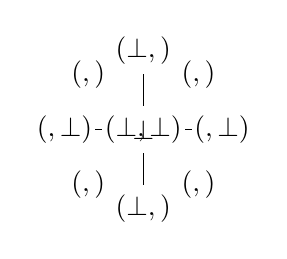
\begin{tikzpicture}

    \begin{scope}
        \myGlobalTransformation{0}{-0.4};
        \node (bottom) at (0,0) {$\bot$};

        \myGlobalTransformation{0}{0.9};
        \node (botbot) at (0,0) {$(\bot,\bot)$};

        \myGlobalTransformation{0}{3};
        \node (trubot) at (-1,0) {$(\tru,\bot)$};
        \node (bottru) at (0,1)  {$(\bot,\tru)$};
        \node (falbot) at (1,0)  {$(\fal,\bot)$};
        \node (botfal) at (0,-1) {$(\bot,\fal)$};

        \myGlobalTransformation{0}{5.5};
        \node (trutru) at (-0.7, 0.7) {$(\tru,\tru)$};
        \node (faltru) at ( 0.7, 0.7) {$(\fal,\tru)$};
        \node (falfal) at ( 0.7,-0.7) {$(\fal,\fal)$};
        \node (trufal) at (-0.7,-0.7) {$(\tru,\fal)$};

        \draw (bottom) -- (botbot);

        \draw (botbot) -- (trubot);
        \draw (botbot) -- (bottru);
        \draw (botbot) -- (falbot);
        \draw (botbot) -- (botfal);

        \ddraw{trubot}{trutru};
        \ddraw{bottru}{trutru};
        \ddraw{falbot}{faltru};
        \ddraw{bottru}{faltru};
        \ddraw{trubot}{trufal};
        \ddraw{botfal}{trufal};
        \ddraw{botfal}{falfal};
        \ddraw{falbot}{falfal};

    \end{scope}

\end{tikzpicture}

%\end{document}}
%  \caption{Two partial orders as Hasse Diagrams}
%  \label{fig:pos}
%\end{figure}

\begin{wrapfigure}[25]{r}{0.4\textwidth} %\begin{figure}\begin{figure}[h!]
\begin{center}
\vspace{-30pt}
%\documentclass[10pt]{article}
\newcommand{\myGlobalTransformation}[2]
{
    \pgftransformreset;
    \pgftransformcm{1.6}{0}{0.65}{0.5}{\pgfpoint{#1cm}{#2cm}}
}

\newcommand\tru{\hs{T}}
\newcommand\fal{\hs{F}}

\newcommand\ddraw[2]{
        \draw[-,line width=3pt,draw=white] (#1) -- (#2);
        \draw (#1) -- (#2);
}

%\begin{document}
%\pagestyle{empty}

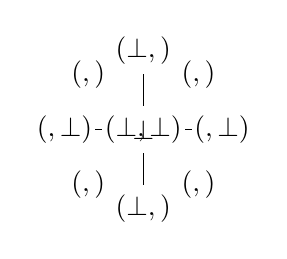
\begin{tikzpicture}

    \begin{scope}
        \myGlobalTransformation{0}{-0.4};
        \node (bottom) at (0,0) {$\bot$};

        \myGlobalTransformation{0}{0.9};
        \node (botbot) at (0,0) {$(\bot,\bot)$};

        \myGlobalTransformation{0}{3};
        \node (trubot) at (-1,0) {$(\tru,\bot)$};
        \node (bottru) at (0,1)  {$(\bot,\tru)$};
        \node (falbot) at (1,0)  {$(\fal,\bot)$};
        \node (botfal) at (0,-1) {$(\bot,\fal)$};

        \myGlobalTransformation{0}{5.5};
        \node (trutru) at (-0.7, 0.7) {$(\tru,\tru)$};
        \node (faltru) at ( 0.7, 0.7) {$(\fal,\tru)$};
        \node (falfal) at ( 0.7,-0.7) {$(\fal,\fal)$};
        \node (trufal) at (-0.7,-0.7) {$(\tru,\fal)$};

        \draw (bottom) -- (botbot);

        \draw (botbot) -- (trubot);
        \draw (botbot) -- (bottru);
        \draw (botbot) -- (falbot);
        \draw (botbot) -- (botfal);

        \ddraw{trubot}{trutru};
        \ddraw{bottru}{trutru};
        \ddraw{falbot}{faltru};
        \ddraw{bottru}{faltru};
        \ddraw{trubot}{trufal};
        \ddraw{botfal}{trufal};
        \ddraw{botfal}{falfal};
        \ddraw{falbot}{falfal};

    \end{scope}

\end{tikzpicture}

%\end{document}
\caption{
    \texttt{(Bool,Bool)} partial order.
    \label{fig:boolboolcpo}
}
\end{center}
\end{wrapfigure} %\end{figure}
For tuples and other constructors that take other data types as
parameters, the ordering is:
\begin{equation*}
\hstup{x_0}{y_0} \sqsubseteq_{(a,b)} \hstup{x_1}{y_1} \text{\quad iff \quad}
x_0 \sqsubseteq_a x_1 \text{\w and \w} y_0 \sqsubseteq_b y_1
\end{equation*}

The Hasse Diagram for the \hs{(Bool,Bool)} values can be seen in
Figure \ref{fig:boolboolcpo}. Here \hs{True} is abbreviated for \hs{T}
and similarly for \hs{False}. It is not flat as the one for \hs{Bool};
it can be seen as three dimensional. On the lowest layer the only
value is $\bot$, on the next layer $\hstup{\bot}{\bot}$. Above that
the tuples with one $\bot$, and finally the total values at the
top.

\vspace{55pt}

\subsection{Monotonicity}
 An important property all safe Haskell functions have is that they are
monotone with respect to this ordering.

\paragraph{Definition} A function $f$ is \emph{monotone} iff

\begin{equation*}
\faa{x}{y} \quad x \sqsubseteq y \quad \Rightarrow \quad f(x) \sqsubseteq f(y).
\end{equation*}

This can be understood in many ways. One way to see it is if you have
two inputs to a function, one containing \emph{less} information that
the other, i.e. more bottoms, it is impossible to return \emph{more}
information from the input with less information.

\newpage

One simple example of a consequence of this is the impossibility to
make a function \hs{isBottom :: a -> Bool}, returning \hs{True} if the
argument is bottom, and \hs{False} otherwise:

\note{rewrite with code}
\begin{align*}
& \hs{isBottom} \w :: \hs{a} \rightarrow \hs{Bool} \\
& \hs{isBottom} \w \bot = \hs{True} \\
& \hs{isBottom} \w x \, = \hs{False}, \qquad x \neq \bot
\end{align*}

\noindent
Since $\bot \sqsubseteq x$ for any $x$, then by monotonicity we must
necessarily have
$$\hs{isBottom} \w \bot \sqsubseteq \hs{isBottom} \w x.$$
Take any non-bottom $x$, and this equation gives
$\hs{True} \sqsubseteq \hs{False}$, which is false. Hence
\hs{isBottom} is not monotone.

\subsection{Continuity}
Another domain theoretic property that Haskell functions have is that
they are continuous. This is a property that gives us insight in how
functions behave on infinite input.  To describe this, we need to
consider the partial order of a data type with infinite values. The
prime candidate \hs{data Nat = Zero | Succ Nat} is used and Hasse
Diagram can be seen in Figure \ref{fig:natcpo}.

\begin{figure}[h]
\centering
\usetikzlibrary{positioning,shadows,arrows}

\def\adots{\mathinner{\mkern2mu\raise\hbox{.}
\mkern2mu\raise4\hbox{.}\mkern1mu
\raise8\vbox{\kern7\hbox{.}}\mkern1mu}}


%\begin{tikzpicture}[scale=10]
%
%  \node (bottom)                          {$\bot$};
%  \node (zero)        [above=of bottom]   {$Zero$};
%  \node (suc bot)     [right=of zero]     {$Suc \, \bot$};
%  \node (suc zero)    [above=of suc bot]  {$Suc \, Zero$};
%  \node (suc suc bot) [right=of suc zero] {$Suc \, (Suc \, \bot)$};
%
%  \draw [-] (bottom) -- (zero);
%  \draw [-] (bottom) -- (suc bot);
%  \draw [-] (suc bot) -- (suc zero);
%  \draw [-] (suc bot) -- (suc suc bot);
%
%\end{tikzpicture}
%
\begin{tikzpicture}[grow'=up,sibling distance=2cm]
\node {$\bot$}
    child {
        node {$\hs{Zero}$}
    }
    child {
        node {$\hs{Succ} \, \bot$}
        child {
            node {$\hs{Succ} \, \hs{Zero}$}
        }
        child {
            node {$\hs{Succ} \, (\hs{Succ} \, \bot)$}
            child {
                node {$\hs{Succ} \, (\hs{Succ} \, \hs{Zero})$}
            }
            child {
              node {$ ^{ ^{\adots}}$}
              child [edge from parent/.style={draw=white}] { }
              child {
                node {$\hs{inf}$}
              }
            }
        }
    }

\end{tikzpicture}


\caption{
    The (complete) partial order for \texttt{Nat}, with \hs{inf = Succ inf.}
    \label{fig:natcpo}
}
\end{figure}

At the top we have the infinite value \hs{inf}, defined in Haskell as
\hs{inf = Succ inf}. Here \hs{inf} is the \emph{limit} of an
$\omega$-chain, i.e a chain with the same number of elements as
$\omega$, the natural numbers. The chain is:

\begin{equation*}
\bot \sqsubseteq
\hs{Succ} \, \bot \sqsubseteq
\hs{Succ} \, (\hs{Succ} \, \bot) \sqsubseteq
\hs{Succ} \, (\hs{Succ} \, (\hs{Succ} \, \bot)) \sqsubseteq
\cdots
\end{equation*}

This chain could succinctly be written $\langle \hs{Succ}^n \, \bot
\rangle_{n \in \omega}$.  Here $\hs{Succ}^n$ means $n$ applications of
the \hs{Succ} constructor. The limit is written $\lub{n \in
  \omega}(\hs{Succ}^n \, \bot)$ and is equal to \hs{inf}, where
$\lub{}$ is the least upper bound. All elements in the chain satisfy
the property of being less than or equal to the limit: $\hs{Succ}^n \,
\bot \sqsubseteq \hs{inf}$.

A partial order is a complete partial order iff there is a limit for
every $\omega$ chain. All data types in Haskell are complete partial
orders\footnote{Notice that the data type \hs{data StrictNat = Zero |
    Succ !StrictNat} is flat and therefore complete.}. Now we can
define continuity.

\paragraph{Definition} A function $f$ is \emph{continuous} iff it is
monotone and preserves the $\lub{ }$ of all $\omega$-chains: i.e.
assume any chain $\langle x_n \rangle_{n \in \omega}$, then:

\begin{equation*}
\lub{n \in \omega} \, (f \, x_n) \eq f \, (\lub{n \in \omega} \, x_n)
\end{equation*}

Just as with monotonicity, there are several ways to interpret
this. One way is to say that what a function does on a chain, it must
also do on the chain's limit, as with \hs{map} on increasingly longer
lists. Another is to say that a function cannot produce finite output by
inspecting infinite input: there is no function
\hs{isFinite :: [a] -> Bool} returning \hs{True} on finite lists and
\hs{False} on infinite lists. On the increasing chain
$$ \bot \sqsubseteq x_0 \hs{:} \bot \sqsubseteq x_0 \hs{:} x_1 \hs{:} \bot
\sqsubseteq \cdots$$
the function \hs{isFinite} returns \hs{True} (or $\bot$), but the
limit should return \hs{False}, so this is not a continuous function.

An interesting formulation of Church's Thesis in terms of continuity
is given by Plotkin \cite{domains}:

\begin{center}
\emph{A function is continuous iff it is physically feasible.}
\end{center}

This means that all computable functions are contiuous, and the other
way around. The conclusion for us is that all Haskell functions are
continuous.

\subsection{Unsafe Haskell}
In GHC, you can use \hs{unsafePerformIO} and \hs{catch} from
\hs{Control.Exception} and other tricks to unsafely catch errors
(bottoms). With this machinery it is possible to write a function
\hs{isBottom :: a -> Bool} to catch calls to \hs{undefined}, pattern
match failures, etcetera. In addition, some non-termination some can
also be catched in Haskell because of the \emph{blackhole} run time
object that replaces a \emph{thunk} that is being currently
evaluated. It does not and indeed cannot cover all non terminating
functions because of the undecidability of the Halting problem.

The domain theoretic results remain; one can see $\bot$ as another,
albeit inconveniently inspected, constructor to every data type. All
patterns are exhaustive: every function has an implicit match any
pattern to $\bot$.  Then we add a \emph{true} bottom to the domain
denotes the uncatchable bottoms; undeterminable non termination. With
this setting all Haskell functions are continuous with respect to the
\emph{true} bottoms. But for the rest of this thesis, we shall only
consider pure and safe Haskell functions.

\subsection{Monotonicity as Verification}

Continuity is a concept that is hard to express in first order logic:
it in not able to express countability. We can come close with an
axiomatization of set theory, but we leave that issue and focus on
monotonicity. A way to verify the translation is to add axioms to the
generated theory describing the $\sqsubseteq$ relation, and axioms
that asserts that each function is monotone. An automated theorem
prover could not easily show that it is a satisfiable theory since it
will normally only have infinite models. However, a long run without
any counter model could be seen as a witness for a successful
translation in this respect.


\section{Future Work}

Haskell is a big language, and translating it all in one go is a
daunting task. Therefore, some restrictions were settled to be able to
focus on proving rather than translating.  The goal was to add enough
of the Haskell language to enable to prove interesting properties, but
much of the widely available sugar in Haskell was omitted since it
does not add extra expressibility.

Some parts of Haskell that are not supported are list
comprehensions and do-notation can be added by its rewriting rules.
\hs{Type} definitions should be unrolled , so they could be used in
the signature for properties. Type classes is probably the most
interesting thing to add, and an approach would be to use dictionary
passing, and inline for concrete types. However, more type information
would be needed but it is possible that much of it could be extracted
from example GHC. Since type classes are not not translated,
higher-kinded type variables are neither.

Another interesting but omitted feature are the built-in types like
\hs{Int}, \hs{Integer}, \hs{Double}, \hs{Char}, etc. For \hs{Integer}
appropriate axioms could be added that hold for $\mathbb{Z}$, the
canonical infinite discretely ordered commutative ring. For the other
data types it is as simple because of different bit sizes and overflow
and precision errors.

Syntactic features for controlling lazy and strict evaluation like
irrefutable patterns, \hs{seq} and bang patterns, and richer pattern
matching in form of pattern bindings are discussed below, but it
should be noted that it is already possible to prove a lot of
interesting Haskell properties, it is far from able to prove things
about bigger Haskell projects which usually use a richer part of the
language.

\subsection{Irrefutable Patterns and Pattern Bindings}

Irrefutable patterns can be defined in terms of strict projections,
like those that already exist (\hs{fst}, \hs{snd}, \hs{head},
\hs{fromJust}, and so on.) Each irrefutable pattern is translated to a
constant, and when you use the variables in the pattern, you translate
it to appropriate use of strict projections. One example is the
translation of the \hs{uncurry} function:

\begin{code}[mathescape]
uncurry f ~(x,y) = f x y        $\Leftrightarrow$      uncurry f t = f (fst t) (snd t)
\end{code}

\noindent
The irrefutable pattern \verb:~(x,y): is replaced with the new constant
\hs{t}, and in the body of the function, \hs{x} is replaced with the
strict projection \hs{fst t}, and similarly for \hs{y}.

Top level patterns, more specifically called pattern bindings, can
also be written in terms of such strict projections. The whole pattern
is replaced with a constant, and when the variables from the pattern
are used, you again replace it with strict projections. This is how it
could look for a simple \hs{fromJust . lookup} implementation:

\begin{code}[mathescape]
unsafeLookup x xs = v           $\Leftrightarrow$      unsafeLookup x xs = fromJust t
  where Just v = lookup x xs            where t = lookup x xs
\end{code}

The strict projections would not rely on the user having \hs{fst} or
\hs{fromJust} in scope, they can automatically be generated by
inspection of the data type definition.

\subsection{Bang Patterns and seq}

The encoding for bang patterns and \hs{seq} is also straightforward,
say you want to define seq with bang patterns, you would have

\begin{code}
seq :: a -> b -> b
seq !x y = y
\end{code}

The axioms needs to ensure that if \hs{x} evaluates to $\bot$, then
\hs{seq x} also evaluates to $\bot$. The two axioms for this functions are:
\begin{align*}
\rom{1} \qquad & \fa{y}    seq(\bot,y) \eq \bot \\
\rom{2} \qquad & \faa{x}{y} x \neq \bot \rightarrow seq(x,y) \eq y
\end{align*}

Either you implement bang patterns in this fashion, or you do the same
translation as GHC for bang patterns: for each strict variable, you
add a \hs{seq} for that variable for the expression of that pattern,
and you simply add the axioms for \hs{seq} to the theory if the
program uses it or bang patterns. This also works for data types with
strictness fields.

\subsection{Pattern Guards}

Patterns guards is a GHC specific extension to Haskell, allowing
arbitrary pattern matching on an expression in a guard. An example is
this elaboration of the \hs{lookup} function from the \hs{Prelude},
which applies a function to the element, if found:

\begin{code}
transformLookup :: Eq k => k -> [(k,v)] -> (k -> v -> b) -> Maybe b
transformLookup k xs f | Just v <- lookup k xs = Just (f k v)
                       | otherwise             = Nothing
\end{code}

\noindent
If the lookup returns \hs{Just}, you already have the value \hs{v}
bound and can use it in the expression for this pattern. This is not
at all unlike the normal guards, they are a special case of pattern
guards: the guard \hs{f x | p x} is expressed as
\hs{f x | True <- p x}. The translation of guards currently checks if
\hs{p x} is \hs{True}, and then ``picks'' this branch, or $\bot$ and
then ``returns'' $\bot$. You could just as well do this for other
constructors, you just need to add bottoms in the guard branches just
as is currently done for ordinary patterns.



\chapter{Proof Techniques}
\label{ch:proofs}

The proof developed in this thesis is called \hs{hip}, the Haskell
Inductive Prover. To use it, properties are inserted to the source
code where the definitions of the relevant functions are. As an
example, this is how the associativity of list concatenation can be
entered:

\begin{code}
import AutoPrelude

prop_app_assoc :: [a] -> [a] -> [a] -> Prop [a]
prop_app_assoc xs ys zs = xs ++ (ys ++ zs) =:= (xs ++ ys) ++ zs
\end{code}

\noindent
The arguments are universally quantified, so this property means:

\newcommand\append{+\!+}
\begin{equation*}
  \faaa{xs}{ys}{zs} xs \append (ys \append zs) = (xs \append ys) \append zs
\end{equation*}

\noindent
The equality is interpreted as equality on the constructor level: two
values are identified if they are constructed with the same
constructor and their arguments are also equal.

The infix function \hs{=:=} comes from the import, as well as the type
constructor \hs{Prop}. The type signature cannot be omitted as this is
used for some proof techniques.  Using \hs{hip} is then a matter of
saving the file, for instance to \hs{ListProps.hs}, and executing this
statement in your favourite terminal:

\begin{code}
hip ListProps.hs
\end{code}

The program will report to you which proof methods succeeded on proving
this property, if any. In this case, it is provable with all three
inductive techniques.

By importing \hs{AutoPrelude} the properties in the file are also
testable with QuickCheck, given that there are appropriate \hs{Eq} and
\hs{Arbitrary} instances provided.

The rest of this chapter explains the different proof methods
supported in this tool. Some properties are a direct consequence from
the definitions in your file. How to prove such properties is
described in Section \ref{sec:equality} about definitional
equality. The three other techniques uses induction in different
ways. Structural induction is explained in Section
\ref{sec:induction}, which uses the structure of the data types a
property quantifies over. Another method which does induction on the
recursive structure of the program is Fixed point induction,
introduced in Section \ref{sec:fixpoint}. A more subtle way of
induction is used in the Approximation Lemma, Section
\ref{sec:approx}, where the structure of the data type of the equality
is approximated.

\pagebreak

% Definitional Equality -------------------------------------------------------

\section{Definitional Equality}
\label{sec:equality}

Some properties cannot or need not use induction or some more
sophisticated technique, since they are true by definition. Examples
are properties for fully polymorphic functions such as this definition
of \hs{id} in the SK-calculus:

\begin{code}
s f g x = f x (g x)
k x y = x
id x = x

prop_skk_id :: Prop (a -> a)
prop_skk_id = s k k =:= id
\end{code}

The generated conjecture stated with function pointers as this:

\begin{equation*}
\app{ (\app {\ptr{s}} {\ptr{k}} )
    }{\ptr{k}} = \ptr{id}
\end{equation*}

However, it is not provable in this form. The next section will solve this.

\subsection{Extensional Equality and \texttt{seq}}

To prove the previous property we also need to have extensional
equality, postulated with this following axiom:

\begin{equation*}
\faa{f}{g} (\fa{x} \app{f}{x} = \app{g}{x}) \rightarrow f = g
\end{equation*}

\noindent
which identifies function pointers and functions composed with $@$.
One problem with extensional equality in Haskell, is that the presence
of \hs{seq} weakens it. \hs{seq} is a built in function with the
following behaviour:

\begin{code}[mathescape]
seq :: a -> b -> b
seq $\bot$ y = $\bot$
seq x y = y$, \qquad x \neq \bot$
\end{code}

It forces the first argument to weak head normal form and returns the
second. For our purposes, it is only important if the first argument
is $\bot$, then the function also returns this as it is strict in its
first argument. With \hs{seq} it is possibly to distinguish between
these two functions, breaking extensional equality since they are
otherwise observationally equal:

\begin{code}[mathescape]
f = $\bot$
g = \x -> $\bot$
\end{code}

Because \hs{seq f ()} evaluates to $\bot$, and \hs{seq g ()} evaluates
to \hs{()}, but on any argument \hs{f} and \hs{g} gets, they both
return $\bot$. Here we also need an extra axiom, which says that
anything applied to $\bot$ is $\bot$:

\begin{equation*}
\fa{x} \app{\bot}{x} = \bot
\end{equation*}

However, \hs{seq} is the only function that can tell such functions
apart, so we will ignore its presence in Haskell.  In the future,
there could be added as a switch \hs{--enable-seq}, which weakens
extensional equality appropriately.

If extensional equality is assumed we also have the property that
\hs{Prop (a -> b)} is equivalent to \hs{a -> Prop b}, by letting the
property have an extra argument that is applied to the left and right
hand side of the equality. This has two benefits. Firstly, it can
trigger other proof methods should \hs{a} or \hs{b} be concrete types
(the former for induction and the latter for approximation
lemma). Secondly, for many properties the extensionality axiom which
introduces extra steps in the proof search is not needed.

The property about \hs{s k k} is then instead translated to:

\begin{equation*}
\fa{x} \fn{s}(\ptr{k},\ptr{k},x) = \fn{id}(x)
\end{equation*}

This gives a little less unnecessary overhead to the theorem provers.

\subsection{Future Work: Concrete Concerns}
\label{sec:concreteconcerns}

This only works on non-concrete types because of the way bottoms are
added. One example of such a problem is this standard definition of
\hs{\&\&}, and a property stating its right identity:

\begin{code}
True  && a = a
False && _ = False

prop_or_right_identity :: Bool -> Prop Bool
prop_or_right_identity x = x && False =:= x
\end{code}

The translation of \hs{\&\&} makes any element in the domain that is not
the introduced constants $\fn{false}$ or $\fn{true}$ for \hs{Bool}'s
constructors, equal $\bot$. Now consider the translation of the
property:

\begin{equation*}
\fa{x} x \, \fn{\&\!\&} \, \fn{true} = x
\end{equation*}

Now this is false, take a model with another element $\diamond$ in the
domain:

$$\diamond \, \fn{\&\!\&} \, \fn{true} = \bot$$

The consequence of this is that the proof principle of definitional
equality is only used on abstract types, rather than polymorphic, as
they cannot be strict. Do not fear: the property above is trivially
proved by induction, as induction for \hs{Bool} and other non
recursive data types degenerate into mere case enumeration. However,
it can only be seen as a meta theorem as it cannot simply be added as
a lemma in the theory. This phenomena is described in more detail in
Section \ref{sec:thmlemmas}. Structural induction is described in
detail in the next section.




% Structual Induction ---------------------------------------------------------

\section{Structural induction}

Any non-recursive, or more importantly recursive data type gives rise
to induction schemata.

\footnote{Haskell's natural numbers are of course also cluttered with
  elements that are not natural numbers, such as $\bot$, but also the
  infinite ``natural number'' defined by \hs{infinite = Succ infinite}}
, defined the usual way in Haskell by \hs{data Nat = Zero | Succ Nat}
yields this induction axiom schema:

\begin{mathpar}
  \inferrule*
     {
       P(\fn{Zero})
       \\
       \fa{x} P(x) \rightarrow P(\fn{Succ}(x))
     }
     { \fa{x} P(x) }
\end{mathpar}


% Fixpoint Induction ----------------------------------------------------------

\section{Fixed Point Induction}
\label{sec:fixpoint}

Structural induction is applicable when at least one argument is of a
concrete type, such as lists or trees. There are also properties where
all arguments are of abstract types. A canonical example is the
map-iterate property::

\begin{equation*}
\faa{f}{x} \hs{map} \w f \w (\hs{iterate} \w f \w x) \eq
           \hs{iterate} \w f \w (f \w x)
\end{equation*}

Here $f$ is any function of type $a \rightarrow a$, and $x$ is a value
of type $a$. This example is further investigated in Section
\ref{sec:mapiter} below, but it is already clear that this property
cannot be proved with structural induction since there is no argument
of a concrete type.

Enter fixed point induction. It gives a way of performing induction on
the recursive structure of the program. In short, if the property
regards a function $f$, the hypothesis is that the property holds for
all the recursive calls in the definition of $f$, and the goal is to
prove that it holds for $f$. The origin of the name is the use of the
fixed point combinator, which is traditionally defined in Haskell as
\hs{fix}:

\begin{code}
fix :: (a -> a) -> a
fix f = f (fix f)
\end{code}

Fixed point induction can prove properties about \hs{fix f} for some
\hs{f}, and the next section gives a method to rewrite any recursive
functions in terms of \hs{fix}. Then properties about recursive
functions in general can be proved by fixed point induction.

The fixed point in question is the solution of the fixed point
equation $x = f \w x$. The function \hs{fix} solves this equation:
substitute $x$ for $\hs{fix} \w x$, then the left side evaluates to $f
\w (\hs{fix} \w f)$ in one step, which is then equal to the right
side. This is the origin of the name of the combinator \hs{fix}: this
is a fixed point of the equation, furthermore it is the least fixed
point \citep{domains}.

\begin{comment}
The domain theoretic approach is to say that
$\hs{fix} \w f \eq \lub{n}(f^n \bot)$, where $f^n \bot$ is $n$
applications of $f$:
\begin{equation*}
f^n \bot \eq \underbrace{f (f (\cdots (f}_{n \w \mathrm{copies \w of} \w f}} \bot) \cdots))
\end{equation*}
This corresponds to a potentially infinite, countable unrolling of $f$.
It is easy to verify that $\langle f^n \bot\rangle_{n\in\omega}$ is a
$\sqsubseteq$-chain by induction on $n$, and that this is the least
pre-fixed point of $f$ is also showed by induction: Assume there
is another pre-fixed point $\theta$, thus satisfying
$\theta \eq f \w \theta$. The base case is
$\bot \eq f^0 \bot \sqsubseteq \theta$, trivially satisfied since
$\bot$ is the least element. For the step case, assume that
$f^n \bot \sqsubseteq \theta$, and we get the conclusion
$f^{n+1} \bot = f (f^n \bot) \sqsubseteq f \w \theta = \theta$ as desired.
\end{comment}

\subsection{Rewriting Functions in Terms of \texttt{fix}}

Any self-recursive function can be rewritten in terms of
\hs{fix} \citep{YMcAdam}. This is a mechanical translation which simply prepends a new
argument which is used for each recursive call of the function. This
is exemplified for the \hs{map} function in Figure \ref{code:mapfix}
below. A new argument \hs{m} is introduced and the recursive call uses
\hs{m} instead of \hs{map}.

\begin{figure}[h!]
\centering
\begin{minipage}[b]{6cm}
\begin{code}[mathescape]
map :: (a -> b) -> [a] -> [b]
map f (x:xs) = f x : map f xs
map f [] = []
$\newline$
$\newline$
\end{code}
\end{minipage}
\hspace{10pt}
\begin{minipage}[b]{6cm}
\begin{code}
map' m f (x:xs) = f x : m f xs
map' m f [] = []

map :: (a -> b) -> [a] -> [b]
map = fix map'
\end{code}
\end{minipage}
\caption{The standard definition of \texttt{map} and a definition in
  terms of \texttt{fix}
\label{code:mapfix}
}
\end{figure}

The correctness of the translation of \hs{map} in Figure
\ref{code:mapfix} is immediate: \hs{fix map'} evaluates to \hs{map'
  (fix map')} by the definition of \hs{fix}, which means that the
recursive function \hs{m} is \hs{fix map'}. By construction it is then
equal to the original definition of \hs{map}.

Generally, for a function \hs{f} with $n \geq 0$ arguments $\hs{x}_1$
to $\hs{x}_n$ and a body $e[\hs{f},\hs{x}_1,\ldots,\hs{x}_n]$ with
these variables free, the definition in terms of \hs{fix} is:

\begin{align*}
& \hs{f } \hs{x}_1 \ldots \hs{x}_n \hs{ = } e[\hs{f},\hs{x}_1,\ldots,\hs{x}_n] & \Rightarrow &&& \fixhsb{f} \w \fixhsw{f} \w \hs{x}_1 \ldots \hs{x}_n \hs{ = } e[\fixhsw{f},\hs{x}_1,\ldots,\hs{x}_n] \\
&                                                                     &             &&& \hs{f = fix} \w \fixhsb{f}
\end{align*}

The funny notation with filled and outlined circles carry some
meaning. The black dot in $\fixhsb{f}$ indicates that this function
has an implementation, mnemonic filled with implementation. The
outlined circle in $\fixhsw{f}$ means that this function does not have
any implementation, it is empty. However, when $\hs{fix }\fixhsb{f}$
unrolls this will replace $\fixhsw{f}$.

\begin{comment}
This translation needs to be carried out with some care, since for $f
\, \overline{x} = e(\overline{x},f)$, it is also possible that $f$ is
called in bodies of other functions. These are of two kinds: either
this function is also called from $f$, making it recursive, or another
function which is not called from $f$, but makes use of $f$
anyway. The first example, with a recursive call, the body needs to be
edited so $f$ becomes translated (to $\bot$, $\unfix{f}$ or
$\tofix{f}$), and the second case should use the original $f$. The
transitive closure of the call graph is calculated, and every
appropriate calls of $f$ are replaced.
\end{comment}

%\noindent
As promised, fix point induction proves properties about a function written in terms
of \hs{fix}, and its inference rule will be stated in the next section.

\subsection{Inference Rule}

Fixed point induction can show a property $P$ about \hs{fix f} for
some function \hs{f}. The base case is to show that $P$ holds when the
function is replaced with $\bot$, which corresponds to zero
``unrolls'' of the function. For the step case, assume $P$
holds for a function $x$, and the goal is to show $P(\hs{f} \w x)$.
Intuitively, we can see $x$ as a number of ``enrolling'' of the
function and we need to show for the next. Moreover, it can also be
seen as $x$ corresponds to all the recursive occurrences in the body of
the function, and we need to show it for the real function.

Using the notation from \cite{corecursive}, we now state its
inference rule:


\begin{mathpar}
  \inferrule*
     {
       P(\bot)
       \\
       P(x) \rightarrow P(f \w x)
       \\
       P \w \mathrm{admissible}
     }
     { P(\fn{fix} f) }
\end{mathpar}

Admissible predicates was introduced in Section \ref{sec:admissible},
and just as structural induction with the bottom base case, this
induction technique also has the admissibility requirement on the
predicate. Again, predicates from equality properties are admissible.

An interesting property of fixed point induction is that it does not
care about types. Indeed, it works in an untyped setting. In addition,
it can exploit arbitrary recursive structures of the function. A
caveat is that it can only prove properties that must hold for
infinite and partial values.

Fixed point induction is a consequence of induction of natural
numbers. The proof for this relies on the fact that $\lub{n}(f^n \w
\bot) \eq \hs{fix} \, f$, where $f^n$ is $n$ self-applications of
$f$. This is true since \hs{fix} is defined as $f$ applied to it
self. The proof also uses induction over natural numbers and that $f^0
\w \bot \eq \bot$, and the admissibility of $P$. Proof:

\begin{align*}
P(\bot) & \wedge \fa{x} P(x) \rightarrow P(f x) \\
\desclra{$f^0 \w \bot \eq \bot$} \\
P(f^0 \w \bot) & \wedge \fa{x} P(x) \rightarrow P(f x) \\
\descra{instantiation of $x$ to $f^n$} \\
P(f^0 \w \bot) & \wedge \fa{n} P(f^n \w \bot) \rightarrow P(f^{n+1} \w \bot) \\
\descra{induction over $\mathbb{N}$} \\
\fa{n} & P(f^n \w \bot) \\
\descra{\textit{P} admissible} \\
& P(\lub{n}(f^n \w \bot)) \\
\descra{definition of \hs{fix}} \\
& P(\hs{fix} \w f) \\
\end{align*}

\noindent
One reason to introduce fixed point induction is to avoid the natural
numbers in $\fa{n} P(f^n \bot)$ to prove $P(\hs{fix} \w f)$.

The necessary theory ought to be explained by now, so the next section
shows how to apply fixed point induction on the example in the
introduction.

\subsection{Example: map-iterate}
\label{sec:mapiter}

For properties that do not have any arguments with a concrete type,
structural induction is not applicable. The Haskell function
\hs{iterate} is a that makes an infinite list from a seed, by repeated
application of a function, i.e \hs{iterate f x} is the list
 \hs{x:f x:f (f x):}$\cdots$. It is related to Haskell function
 \hs{map} in the map-iterate property, stated as follows:

\begin{equation*}
\faa{f}{x} \hs{map} \w f \w (\hs{iterate} \w f \w x) \eq
           \hs{iterate} \w f \w (f \w x)
\end{equation*}

\noindent
The standard definition of \hs{map} was given above and \hs{iterate}
is defined as this:

\begin{code}
iterate :: (a -> a) -> a -> [a]
iterate f x = x : iterate f (f x)
\end{code}

The behaviour of \hs{map} is to apply a function to every element of a
list. We see that we cannot use structural induction here, since both
$f$ and $x$ are abstract, but the \hs{map}-\hs{iterate} property can
be proved by fixpoint induction on \hs{iterate}. First, we rewrite
this function in terms of \hs{fix}:

\begin{code}
iterate = fix iter
iter i f x = x : i f (f x)
\end{code}

\noindent
The predicate $P$ is defined to be $P(i) \w \Leftrightarrow \w
\faa{f}{x} \hs{map} \w f \w (i \w f \w x) \eq i \w f \w (f \w x)$.
If the base and the step case is shown $P(\hs{fix iter})$ can be
concluded, which by definition is $P(\hs{iterate})$.

The base case is $P(\bot)$. Since \hs{map} is strict in its second
argument, it is both the left side and right side evaluate to $\bot$.
The for the step case we have to show $P(\hs{i}) \rightarrow
P(\hs{iter i})$.  The proof without explicitly writing out function
pointer applications looks like this:

\begin{align*}
lhs & = \hs{map} \w f \w (\hs{iter} \w \hs{i} \w f \w x)          && \{\textrm{definition of \hs{iter}}\} \\
    & = \hs{map} \w f \w (x \hs{:} \hs{i} \w f \w (f \w x))       && \{\textrm{definition of \hs{map}} \} \\
    & = f \w x \hs{:} \hs{map} \w f \w (\hs{i} \w f \w (f \w x))) && \{\textrm{induction hypothesis} \} \\
    & = f \w x \hs{:} \hs{i} \w f \w (f \w (f \w x)))             && \{\textrm{definition of \hs{iter}} \} \\
    & = \hs{iter} \w \hs{i} \w f \w (f \w x) = rhs
\end{align*}
%\w \faa{f}{x}  & \eq \hs{i} \w f \w (f \w x) \\
%\descra{generalising $x$ to $f \w x$} \\
%\w \faa{f}{x} \hs{map} \w f \w (\hs{i} \w f \w (f \w x)) & \eq \hs{i} \w f \w (f \w (f \w x)) \\
%\descra{substitution} \\
%\w \faa{f}{x} f \w x \hs{:} \hs{map} \w f \w (\hs{i} \w f \w (f \w x)) & \eq f \w x \hs{:} \hs{i} \w f \w (f \w (f \w x)) \\
%\desclra{\defof{\texttt{map}}} \\
%\w \faa{f}{x} \hs{map} \w f \w (x \hs{:} \hs{i} \w f \w (f \w x)) & \eq f \w x \hs{:} \hs{i} \w f \w (f \w (f \w x)) \\
%\desclra{\defof{\texttt{iter}}} \\
%\w \faa{f}{x} \hs{map} \w f \w (\hs{iter} \w \hs{i} \w f \w x) & \eq \hs{iter} \w \hs{i} \w f \w (f \w x) \\
%\end{align*}

Now fixed point induction gives the \hs{map}-\hs{iterate} property.



\begin{comment}
\subsection{Mutually Recursive Functions}

You can also mechanically transform mutually recursive functions to be
defined in terms of \hs{fix}. The functions \hs{even} and \hs{odd}
defined below, which determines if a \hs{Nat} is even, and odd,
respectively, are straightforwardly written by mutual recursion:

\begin{code}
even :: Nat -> Bool           odd :: Nat -> Bool
even Z     = True             odd Z     = False
even (S x) = odd x            odd (S x) = even x
\end{code}

To write these functions in terms of fix, as an additional argument,
the take a tuple of ``non-recursive'' copies of themselves.

\begin{code}
evenToFix :: (Nat -> Bool,Nat -> Bool) -> Nat -> Bool
evenToFix (evenUnFix,oddUnFix) Z     = True
evenToFix (evenUnFix,oddUnFix) (S x) = oddUnFix x

oddToFix :: (Nat -> Bool,Nat -> Bool) -> Nat -> Bool
oddToFix (evenUnFix,oddUnFix) Z     = True
oddToFix (evenUnFix,oddUnFix) (S x) = evenUnFix x
\end{code}

Here the prefix \hs{ToFix} means that it is a function subject to be
\hs{fix}-ed, and \hs{UnFix} means that it is the ``non-recursive''
function. The functions above can now be \hs{fix}-ed by giving the
tuple as an argument to both of them:

\begin{code}
even',odd' :: Nat -> Bool
(even',odd') = fix (\t -> (evenToFix t,oddToFix t))
\end{code}

This encoding makes \hs{even'} denotationally equal to \hs{even} and
the same relation hols for \hs{odd'} and \hs{odd}.
\end{comment}

\subsection{Simplification}

The mechanical translation introduced above for self-recursive
functions introduces a new function with an additional argument, the
``non-recursive'' version of itself. The generated first order
function would use the new argument as a function pointer, which in
turn means a lot of use of the $\appfn$. This can be seen in the cons
case for \hs{map}:

\begin{align*}
  \faaa{m}{x}{xs} \fn{map'}(m,x\fn{:}xs) = (\app{f}{x}) \fn{:} (\app{(\app{m}{f})}{xs})
\end{align*}

This gives unnecessary overhead to the automated theorem provers.
There is another approach. It avoids introducing these function
pointers and the additional argument to every function. Consider the
translation of a function \hs{f} with the same setting as before: $n
\geq 0$ arguments $\hs{x}_1$ to $\hs{x}_n$ and a body
$e[\hs{f},\hs{x}_1,\ldots,\hs{x}_n]$ with these variables free,
instead this translation is made:

\begin{align*}
& \hs{f } \hs{x}_1 \ldots \hs{x}_n \hs{ = } e[\hs{f},\hs{x}_1,\ldots,\hs{x}_n] & \Rightarrow &&& \fixhsb{f} \w \hs{x}_1 \ldots \hs{x}_n \hs{ = } e[\fixhsw{f},\hs{x}_1,\ldots,\hs{x}_n] \\
\end{align*}

Two new functions are introduced to the vocabulary: $\fixhsb{f}$ and
$\fixhsw{f}$. The empty circle $\unfix{}$ describes that this function
is empty (lacks implementation,) and the filled circle $\tofix{}$
means that this function has an implementation. This implementation is
in terms of the unfilled version. The fixed point induction schema can
now be stated using these functions:

\begin{mathpar}
  \inferrule*
     {
       P(\bot)
       \\
       P(\unfix{f}) \rightarrow P(\tofix{f})
       \\
       P \, \mathrm{admissible}
     }
     { P(f) }
\end{mathpar}

\noindent
The empty circle in $\unfix{f}$ indicates that it does not have any
implementation, but the induction hypothesis is asserted for it. The
induction conclusion is to prove the property for $\tofix{f}$, where
the recursive call to $f$ is replaced with $\unfix{f}$. This
simplification is done since it is better suited for the theorem
provers.

Further, it is now necessary to ``inline'' the predicate in the
generated theory. The reason is that $\fixb{f}$ and $\fixw{f}$ are
first order functions rather than expressible as pointers, and
predicates that quantify over functions are not first order
expressible. Such ``inlining'' is also beneficial for theorem provers
as unnecessary predicates are not introduced to the theory.

\paragraph{Mutually recursive functions} It is also possible to
rewrite a group of mutually recursive functions by packing the
``non-recursive'' copies of themselves in a tuple. The inference rule
for two functions at the same time, possibly mutually recursive then
looks like this:

\begin{mathpar}
  \inferrule*
     {
       P(\bot,\bot)
       \\
       P(\unfix{f},\unfix{g}) \rightarrow P(\tofix{f},\tofix{g})
       \\
       P \, \mathrm{admissible}
     }
     { P(f,g) }
\end{mathpar}

\noindent
This also works when the functions are not mutually recursive. An
example is the map-iterate property which can be proved by fixating
both \hs{map} and \hs{iterate}.

\subsection{Erroneous Use of Fixed Point Induction}

It is crucial that $P$ is admissible to avoid deriving falsities. This
section gives a simple example of what can happen otherwise. Recall
the definition of the infinite natural number:

\begin{code}
inf = Succ inf
\end{code}

\noindent
A predicate that is not admissible will deliberately be used to
``prove'' that $\hs{inf} \neq \hs{Succ inf}$.  The predicate is $P(x)
\Leftrightarrow x \neq \fn{succ}(x)$. Furthermore, \hs{inf} is
translated to first order logic and rewritten in terms of $\unfix{}$ and
$\tofix{}$, as introduced in the previous section:

\begin{equation*}
\tofix{\fn{inf}} = \fn{succ}(\unfix{\fn{inf}})
\end{equation*}

\noindent
Now we proceed by ``fixed point induction''. Base case: $\bot \neq
\fn{succ}(\bot)$ is true by the axioms of disjoint constructors. Step
case: assume $\unfix{\fn{inf}} \neq \fn{succ}(\unfix{\fn{inf}})$.
Injectivity of $\fn{succ}$ gives $\fn{succ}(\unfix{\fn{inf}}) \neq
\fn{succ}(\fn{succ}(\unfix{\fn{inf}}))$.  By the definition of
$\tofix{\fn{inf}}$, which is then equal to the goal $\tofix{\fn{inf}} \neq
\fn{succ}(\tofix{\fn{inf}})$.

The conclusion $\hs{inf} \neq \hs{Succ inf}$ is clearly nonsense as it
directly contradicts the definition of $\hs{inf}$! A consequence of
this example is that inequality is in general not admissible.

%\end{comment}

\subsection{Candidate Selection}

Faced with the following property saying that if you drop $n$ elements
from a list the length of this is the same as the length of the
original list minus $n$, which functions should one do fixed point
induction on?

\begin{code}
prop_length_drop :: [a] -> Nat -> Prop Nat
prop_length_drop xs n = length (drop n xs) =:= length xs - n
\end{code}

\noindent
The answer is to do fixed point induction on \hs{drop}, and on
\hs{-}. So far no better way to tackle this is used than to try fixed
point induction on all subsets of recursive functions mentioned in the
property.

\subsection{Future Work}

Just as with structural induction, it is also possible to use fixed
point in more than one ``depth'', giving for instance this inference
rule:

\begin{mathpar}
  \inferrule*
     {
       P(\bot)
       \\
       P(f \w \bot)
       \\
       P(x) \wedge P(f \w x) \rightarrow P(f \w (f \w x))
       \\
       P \w \mathrm{admissible}
     }
     { P(\fn{fix} f) }
\end{mathpar}

It is also possible to use such an encoding as in ``Automated depth''
in Section \ref{sec:futind} to let the theorem prover determine the
depth. As an example, the map-iterate property impossible to show with
\hs{map} redefined to \hs{doublemap}, defined below, with ordinary one
depth fixed point induction.

\begin{code}
doublemap :: (a -> b) -> [a] -> [b]
doublemap f []       = []
doublemap f [x]      = [f x]
doublemap f (x:y:zs) = f x : f y : doublemap f zs
\end{code}

\noindent
Although \hs{doublemap} is behaviourally equivalent to \hs{map} on total
lists, it makes the induction hypothesis in fixed point induction too
weak.


An issue with the candidate selection is that is some selections are
immediate dead ends. An example is fixating functions on only one side
of the equality, then the base case will generally never succeed
unless the other side is constant bottom. A heuristic to find good
candidates would be beneficial.


% Approximation Lemma ---------------------------------------------------------

\section{Approximation Lemma}
\label{sec:approx}

The approximation lemma is another standard technique for proving
properties about corecursive programs. Just like fixed point induction
it can be used with functions that are produce infinite values, like
\hs{repeat} and \hs{iterate}, out of abstract values making structural
induction impossible \cite{corecursive}, but the approximation lemma
usually supersedes lemma fixed point induction since it is much
simpler to apply.

The approximataion lemma supersedes the classical take lemma
\cite{introfp} by being easier to apply and generalize: unlike the
take lemma, it can be applied to equalities of any polynomial data
type \cite{genapprox}. The definitions of \hs{take} and \hs{approx}
can be seen in Figure \ref{code:takeapprox}.

%\note{write this as Haskell code? \newline (those \hs{Nat} are actually $\mathbb{N}$)}
\begin{figure}[h!]
\centering
\begin{minipage}[b]{6.2cm}
\begin{code}
take :: Nat -> [a] -> [a]
take Zero    _      = []
take (Suc n) []     = []
take (Suc n) (x:xs) = x : take n xs
\end{code}
\end{minipage}
\hspace{10pt}
\begin{minipage}[b]{6.7cm}
\begin{code}
approx :: Nat -> [a] -> [a]
approx (Suc n) []     = []
approx (Suc n) (x:xs) = x : approx n xs
\end{code}
\end{minipage}
\caption{Definition of \texttt{take} and \texttt{approx}
\label{code:takeapprox}
}
\end{figure}

Whereas \hs{take} approximates a list and ends it with \hs{[]},
\hs{approx} ends it with $\bot$ since the \hs{Zero} case is
omitted. The idea of these techniques is then to show that show that
two lists are equal by showing that their prefix or approximation
coincides for all natural numbers.

\newpage
Now we can state the approximation lemma:

\begin{equation}
\label{eq:approxeq}
xs \, = \, ys \quad \Leftrightarrow \quad \fa{n \in \mathbb{N}} \hs{approx} \, n \, xs = \hs{approx} \, n \, ys
\end{equation}

Equation \ref{eq:approxeq} quantifies over the real natural numbers
(i.e. total and finite), rather than the Haskell naturals. Showing an
equality then amounts to a proof by induction over natural numbers,
and the base case for $0$ is always true by reflexivity, as the
approximation of the two lists is $\bot = \bot$. The right to left
implication is (trivially) true by substitution, and the other
direction hinges on the lemma that better and better approximations
form a chain with limit \hs{id}, as illustrated in Equation
\ref{eq:approxchain} below.

\begin{equation}
\label{eq:approxchain}
\hs{approx} \, 0 \,
   \sqsubseteq \,
\hs{approx} \, 1 \,
   \sqsubseteq \,
\cdots
   \sqsubseteq \,
\hs{approx} \, n \,
   \sqsubseteq \,
\hs{approx} \, (\hs{Suc} \, n) \,
   \sqsubseteq \,
\cdots
   \sqsubseteq \,
\hs{id}
\end{equation}

The inclusions in Equation \ref{eq:approxchain} are easily given by
induction on natural numbers and the limit by structural induction on
lists.  For other polynomial data types, this lemma is established by
the structural induction induced on that data type.  The desired
implication is then readily deduced:

\begin{align*}
\xsys{\fa{n} \hs{approx} \, n}{}            \\
\descra{limits}                             \\
\xsys{\lub{n} \, (\hs{approx} \, n}{)}      \\
\desclra{continuity of application}   \\
\xsys{\lub{n} \, (\hs{approx} \, n)}{}      \\
\desclra{Equation \ref{eq:approxchain}} \\
\xsys{\hs{id}}{}                            \\
\desclra{definition of \hs{id}}       \\
\xsys{}{}                                   \\
\end{align*}

\subsection{Example: Mirroring an Expression}

Consider these definitions of a modest but prototypical expression
data type, and its mirroring function:

\begin{code}
data Expr = Add Expr Expr | Value Nat

mirror :: Expr -> Expr
mirror (Add e1 e2) = Add (mirror e2) (mirror e1)
mirror (Value n)   = Value n

prop_mirror_involutive :: Expr -> Prop Expr
prop_mirror_involutive e = e =:= mirror (mirror e)
\end{code}

The type \hs{Expr} does not have a nullary constructor. Then the
\hs{take} lemma would not be usable as there is no such function over
these expressions: the list version returns the empty list \hs{[]} for
the zero case, but there is no such alternative for \hs{Expr}
above. It is important that the limit of approximations is the
identity, and we cannot get this property when trying to generalise
the take lemma.

Furthermore, fixed point induction fails on this property: choosing
either or both occurrences of \hs{mirror} on the right side is
constant bottom for the base case, and the left side is the identity.

We shall now proceed to prove that \hs{mirror} is involutive by the
approximation lemma. The approximation function for \hs{Expr} is
automatically generated, by approximating each self-recursive
constructor, and hence \hs{Value}'s \hs{Nat} is not further approximated:

\begin{code}
approx :: Nat -> Expr -> Expr
approx (Suc n) (Add e1 e2) = Add (approx n e1) (approx n e2)
approx (Suc n) (Value n)   = Value n
\end{code}

\note{Use $\bot$ or bottom in this text?}
Indeed, we also get a third case for $\bot$ which states that the
approximation of $\bot$ is, quite unsurprisingly, $\bot$.
As always in proofs by approximation lemma, we proceed by induction
over natural numbers, and the base case is always trivial: true by
reflexivity as both sides are $\bot$. The step case - which indeed is
the only proof obligation in any proof of this kind - is to prove

this:

\begin{equation*}
\fa{e}  \hs{approx} \, (\hs{Suc} \, n) \, e = \hs{approx} \, (\hs{Suc} \, n) \, (\hs{mirror} \, (\hs{mirror} \, e))
\end{equation*}

An important property of the induction hypothesis is the universal
quantification of the expression $e$, unlike the fixed natural number
$n$:

\begin{equation*}
\fa{e}  \hs{approx} \, n \, e = \hs{approx} \, n \, (\hs{mirror} \, (\hs{mirror} \, e))
\end{equation*}

The proof is by case exhaustion. The case for \hs{Value} and $\bot$
are trivial: \hs{mirror} is strict in its first argument, and
mirroring \hs{Value} twice is the identity, so these cases are both
true by reflexivity. The \hs{Add} case is ever so slightly more
elaborate, and with names shortened to $\hs{app}$ and $\hs{mir}$ the
reasoning is as follows:

\note{$(\hs{Suc} \, n)$ or $(n + 1)$?}
\newcommand{\Adds}[2]{\hs{add} \, #1 e_1 #2 \, #1 e_2 #2}
\newcommand{\Approxn}[0]{\hs{app} \, n \,}
\newcommand{\ApproxSucn}[0]{\hs{app} \, (\hs{Suc} \, n) \,}
\newcommand{\mirmir}[0]{\hs{mir} \, (\hs{mir} \, }
\begin{align*}
\faa{e_1}{e_2}&  \ApproxSucn (\Adds{}{})  = \ApproxSucn (\mirmir \Adds{}{} ))                                                                   \\
                                                                                 \desclra{\defof{\texttt{mirror}}}                                   \\
\faa{e_1}{e_2}&  \ApproxSucn (\Adds{}{})  = \ApproxSucn (\Adds{(\mirmir}{))})                                                                    \\
                                                                                \desclra{\defof{\texttt{approx}}}                                    \\
\faa{e_1}{e_2}&  \Adds{(\Approxn}{)}      = \Adds{(\Approxn(\mirmir}{)))}                                                                        \\
                                                                                \desclra{induction hypothesis twice ($e_1$ and $e_2$)} \\
\faa{e_1}{e_2}&  \Adds{(\Approxn}{)}      = \Adds{(\Approxn}{)}                                                                                  \\
                                                                                \desca{reflexivity}                                              \\
\end{align*}

\subsection{Approximation Lemma is Fixpoint Induction}

This technique is already simple and widely applicable, however it can
further be simplified. Implementing it in this form relies on the
auxiliary structure of Peano natural numbers which also needs to be
added to the theory. This can be removed by the observation that is
expressed as fixed point induction over a recursive form of the
identity function, called \hs{ind} for its close resemblance of
induction. For lists and the \hs{Expr} data type, \hs{ind} can be seen
in Figure \ref{code:ind}.

\begin{figure}[h!]
\centering
\begin{minipage}[b]{5cm}
\begin{code}[mathescape]
ind$_{\texttt{[a]}}$ :: [a] -> [a]
ind$_{\texttt{[a]}}$ [] = []
ind$_{\texttt{[a]}}$ (x:xs) = x:ind$_{\texttt{[a]}}$ xs
\end{code}
\end{minipage}
\hspace{10pt}
\begin{minipage}[b]{8.3cm}
\begin{code}[mathescape]
ind$_{\texttt{Expr}}$ :: Expr -> Expr
ind$_{\texttt{Expr}}$ (Value n) = Value n
ind$_{\texttt{Expr}}$ (Add e1 e2) = Add (ind$_{\texttt{Expr}}$ e1) (ind$_{\texttt{Expr}}$ e2)
\end{code}
\label{code:approx}
\end{minipage}
\caption{Definition of \texttt{ind} for lists and \texttt{Expr}
\label{code:ind}
}
\end{figure}

Each \hs{ind} function constructed in this way is indeed an identity
function, equivalent to the implementation \hs{id x = x} if we
disregard time and space complexity. Now, to prove

\begin{equation*}
e_1 \, = \, e_2
\end{equation*}

we simply use fixed point induction to prove

\begin{equation*}
\hs{ind} \, e_1 \, = \, \hs{ind} \, e_2
\end{equation*}

where \hs{ind} is a such a specialized recursive identity function
over the data type of the equality. With the same translation for
recursive functions as in the fixed point section the axioms of
\hs{ind} for lists are:

\begin{align*}
\rom{1} &&             & \tofix{\fn{ind}}(\fn{nil})   \eq \, \fn{nil}                                                           \\
\rom{2} && \faa{x}{xs} & \tofix{\fn{ind}}(\fn{cons}(x,xs)) \eq \fn{cons}(x,\unfix{\fn{ind}}(xs))                                                \\
\rom{3} && \fa{xs}     & \tofix{\fn{ind}}(xs)        \eq \bot \leftarrow xs \neq \fn{nil} \wedge xs \neq \fn{cons}(\fn{cons_0}(xs),\fn{cons_1}(xs)) \\
\end{align*}

The step case in induction $P(\unfix{id}) \rightarrow P(\tofix{id})$
is then exactly the same strength as the approximation lemma with
natural numbers. We get this simple rule for approximation lemma:

\begin{mathpar}
  \inferrule*
     {
                    \unfix{\fn{ind}} \w e_1 \eq \unfix{\fn{ind}} \w e_2
        \rightarrow \tofix{\fn{ind}} \w e_1 \eq \tofix{\fn{ind}} \w e_2
     }
     {
        e_1 \eq e_2
     }
\end{mathpar}

Just as fix point induction was introduced to reason about chains
without explicitly relying on natural numbers, this follows the same
pattern. This version of the approximation lemma does not rely on natural
numbers.


%\subsection{Implementation} The implementation of approximation lemma
%was the simplest to implement, after definitional equality. First,
%from the type signature from the property, such a recursive identity
%function as above is generated for the data type of the equality. Then
%the lemma $P(\unfix{id})$ is added to the theory, with $P$
%instantiated to the universally quantified equality, and the
%conjecture is $P(\tofix{id})$. The base case need not be proven,
%$P(\bot)$ is always true since it evaluates to $\bot=\bot$.
%\note{Compare this to skolemization for induction? Can $\tofix{id}$ be
%  viewed as a kind of skolemization?}

\subsection{Future Work: Total Approximation Lemma}

It would be nice to adjust the approximation lemma to prove properties
that are true for total and potentially infinite objects, but false
for objects with partial values. One such property is the idempotence
of \hs{nub}. Here is a version of \hs{nub} on booleans, and the said
property about it:

\begin{code}
nub :: [Bool] -> [Bool]
nub (True :True :xs) = nub (True:xs)
nub (False:False:xs) = nub (False:xs)
nub (x:xs)           = x:nub xs
nub _                = []

prop_nub_idem :: [Bool] -> Prop [Bool]
prop_nub_idem xs = nub (nub xs) =:= nub xs
\end{code}

Consider the list \hs{True:False:}$\bot$. One application of \hs{nub}
gives \hs{True:}$\bot$, and two gives $\bot$ immediately. In spite of
this, the property is a truism for finite as well as infinite lists,
provided that there are not bottoms.

The way to enable the approximation lemma to prove such properties is
to add predicates of totality, and add axioms like the following to
the theory:

\begin{align*}
\rom{1} &&             & \neg \, Total(\bot) \\
\rom{2} &&             & Total(\hs{[]}) \\
\rom{3} && \faa{x}{xs} & Total(x) \wedge Total(xs) \rightarrow Total(x\hs{:}xs) \\
\rom{4} && \fa{xs}     & Total(xs) \rightarrow Total(\hs{nub} \, xs) \\
\end{align*}

Though \hs{Total} is an admissible predicate, we want to use it as an
implication, to use fixed point induction on \hs{ind} to prove
something like this:

\begin{equation*}
\fa{xs} Total(xs)\rightarrow \hs{ind} \w (\hs{f} \w xs) = \hs{ind} \w (\hs{g} \w xs)
\end{equation*}

\noindent
However, this is not admissible. We are searching for another
formulation that is.





%% End of Technical Part ------------------------------------------------------


\chapter{Discussion}

\section{Results}

Test suite

% Future work

\chapter{Future work}
\label{ch:future}

The chapter addresses some limitations of our approach and ideas how
to get around them.

\section{Pattern Matching Re-Revisited}
\label{sec:rerevisited}

The current translation of pattern matching is described in Section
\ref{sec:patternsrevisited}. One of the strengths of it is the
translation of wild patterns. Consider this function for equality of a
data type with three elements:

\begin{code}
data Tri = A | B | C

equal :: Tri -> Tri -> Bool
equal A A = True
equal B B = True
equal C C = True
equal _ _ = False
\end{code}

\noindent
The translation adds two more cases that go to bottom, one where the
first argument is bottom, and one where the second one is bottom. All
other values that are not the same \hs{Tri} and not bottom go to
\hs{False}.

If there for models of this function which includes
another value $\diamond$, other values than those of this data type and
bottom, must have $\fn{equal}(\diamond,x) = \fn{false}$, for all non
bottom $x$, including $\diamond$. This is not a problem per se, since the
Haskell source is well typed, and \hs{equal} will not be applied to
anything but \hs{Tri}s and bottoms.

One weakness of that approach is that two functions that are
extensionally equivalent in Haskell are not in the generated theory,
when applied to non sense arguments. An example of this behaviour is
these two implementations of the boolean or function in Figure
\ref{code:or}.

\begin{figure}[h!]
\centering
\begin{minipage}[b]{6cm}
\begin{code}
or :: Bool -> Bool -> Bool
or False b = b
or True  _ = True
\end{code}
\end{minipage}
\hspace{10pt}
\begin{minipage}[b]{6cm}
\begin{code}
or' :: Bool -> Bool -> Bool
or' False b = b
or' _     _ = True
\end{code}
\end{minipage}
\caption{Two definitions of boolean and, \texttt{and} and \texttt{and'}
\label{code:or}
}
\end{figure}

Let us analyse the models of this program in Figure \ref{code:or} with
an additional value $\diamond$ in the domain. The translation makes
$\fn{or}(\diamond,\fn{true}) = \bot$, since there is a wild pattern that
goes to $\bot$. For the other function we have
$\fn{or'}(\diamond,\fn{true}) = \fn{false}$, as the wild pattern already
goes to $\fn{false}$. Because of this differences, the approximation
lemma cannot prove this property. While this is a simple example, it
is easy to imagine more complex cases where different pattern matching
techniques makes no difference to the Haskell program, but to this
translation.

This suggests that wild patterns should be expanded to pattern for all
their constructors, and add a match any pattern that goes to
bottom. This make the the meta theorem
$\faa{x}{y} \fn{or}(x,y) = \fn{or'}(x,y)$ consistent with rest of the
theory.  Further, it would be provable by the approximation lemma, and
in more complex cases with recursive functions, by fixed point
induction. This translation is also assumed to be a little easier to
implement. The down side is that functions such as \hs{equal} above
would generate $O(n^2)$ axioms, where $n$ is the number of constructors for
the data type. The presence of GADTs and other type extensions such as
type families would requite type information and add a lot of complexity.

\section{Lemmas}

For many properties, especially more advanced ones, it is crucial to
be able to use lemmas to obtain a proof. The introduced proof
techniques in this theses are just not strong enough. For structural
induction, it is possible to do induction in more than one depth. This
sometimes make the hypotheses equally strong as the required lemmas,
as in the example of plus commutativity of natural numbers in Section
\ref{sec:genind}. But this approach fails for properties about
multiplication: it is essential to use lemmas about addition.

The concept of adding lemmas is of course quite simple. Assume your
program has two properties \hs{prop\_a} and \hs{prop\_b}, and the
second needs the first as a lemma. If \hs{prop\_a} succeeds, then the
should program just add that property to the theory generated for
\hs{prop\_b}, and try it again. Unfortunately, adding a property to a
theory needs to be carried out with care. For properties that hold for
infinite and partial values it is actually a bit simpler than for
those that are only true for finite values. These settings are
addressed one by one below.

\subsection{Lemmas from Theorems}

One example of a Theorem, a property that holds for partial and
infinite values, is the right identity of \hs{||}, boolean or:

$$\fa{x} x \w \hs{||} \w \fn{false} = x$$

\noindent
Adding this meta theorem to the theory would make it
inconsistent. Again, in a model with an extra value $\diamond$, we have
that $\diamond \w \hs{||} \w \fn{false} = \bot$. However, we can create a
function that forces a value to be a \hs{Bool} or $\bot$ as this:

\begin{align*}
\rom{1} \qquad &&        & \fn{force}(\fn{true})  && = \fn{true} \\
\rom{2} \qquad &&        & \fn{force}(\fn{false}) && = \fn{false} \\
\rom{3} \qquad && \fa{x} & \fn{force}(x)          && = \bot \vee x = \fn{false} \vee x = \fn{true}
\end{align*}

The theory would be consistent with this reformulation of the meta theorem:

$$\fa{x} \fn{force}(x) \w \hs{||} \w \fn{false} = \fn{force}(x)$$

It is easy to generalise $\fn{force}$ beyond booleans. Make it a
binary function with first argument a description of the type. Each
simply kinded type would be given a constant, and higher-kinded types
functions, an example would be $\fn{list}(\alpha)$ for lists of $\alpha$:

\begin{align*}
\rom{1} \qquad && \fa{\alpha}          & \fn{force}(\fn{list}(\alpha),\fn{nil})        && = \fn{nil} \\
\rom{2} \qquad && \faaa{\alpha}{x}{xs} & \fn{force}(\fn{list}(\alpha),\fn{cons}(x,xs)) && = \fn{cons}(\fn{force}(\alpha,x),\fn{force}(\fn{list}(\alpha),xs) \\
\rom{3} \qquad && \faa{\alpha}{xs}     & \fn{force}(\fn{list}(\alpha),xs)              && = \bot  \\
               &&                      & \multicolumn{3}{l}{\vee xs = \fn{nil} \vee xs = \fn{cons}(\fn{cons_0}(xs),\fn{cons_1}(xs))}
\end{align*}

Using functions and predicates effectively to witness type information
has been studied by \cite{sortMonotonicity} and by
\cite{polyMonotonicity}.

Proofs by definitional equality would also benefit from type tags. The
the current limitations are discussed section
\ref{sec:concreteconcerns}. Furthermore, the extensional equality of
the different implementations of the or function in Figure
\ref{code:or} is not provable with approximation lemma with the
current translation. However, stated with $\fn{force}$-tags it should
be possible. This could give us the best of two worlds: minimal
translation of pattern matching and wider applicability of untyped
proof methods.

\subsection{Lemmas from Finite Theorems}

The $\fn{force}$ function from the previous section is not easily
generatised to remove partiality from a value. Another way to do this
is to introduce a predicate $Total$, indicating totality. This is a
way to axiomatise $Total$ for natural numbers:

\begin{align*}
\rom{1} &&        & \neg \, Total(\bot) \\
\rom{2} &&        & Total(\fn{zero}) \\
\rom{3} && \fa{x} & Total(x) \rightarrow Total(\fn{succ}(x))
\end{align*}

As with the $\fn{force}$ function, it could be wise to add an argument
to $Total$ indicating the type, but for the rest of this section we
will only consider the (Haskell) natural numbers. A property such as the
commutativity of plus could be expressed with this meta theorem:

\begin{equation*}
\faa{x}{y} Total(x) \wedge Total(y) \rightarrow x + y = y + x
\end{equation*}

We would also like to express finiteness. Our canonical example of a
an infinite value is the natural number
\hs{inf = Succ inf}. Identification of such cyclic values can be axiomatised:

\begin{equation*}
\fa{x} Cyclic(x) \leftrightarrow (x = \fn{succ}(x) \vee (\ex{y} x = \fn{succ}(y) \wedge Cyclic(y))) \\
\end{equation*}

Because Haskell functions are continuous and finite, every infinite
value is produced from finite information (\hs{repeat}, \hs{iterate},
\hs{enumFrom}), so a predicate $Cyclic$ should be enough for our
purposes. Further, it is clear that $Cyclic(x) \rightarrow Total(x)$.

\pagebreak

We can now define finiteness of a value $x$ as
$Finite(x) \leftrightarrow Total(x) \wedge \neg Cyclic(x)$.  The results
from a function would be necessary to axiomatise to make such axioms
useable. To exemplify why this is not trivial, consider the
complexities of the plus function:

\begin{align*}
\rom{1} && \faa{x}{y} & Finite(x) \wedge Finite(y)                  & \leftrightarrow &&& Finite(x + y) \\
\rom{2} && \faa{x}{y} & Cyclic(x) \vee (Finite(x) \wedge Cyclic(y)) & \leftrightarrow &&& Cyclic(x + y)
\end{align*}

How to prove the status for the return value of a function in terms of
$Finite$, $Total$ and $Cyclic$ for different statuses of the arguments is
an open problem. Possible sources for inspiration is the work by
\cite{exhaustiblesets}, where topological compactness for
data types play a significant r\^{o}le.

\subsection{Speculating Lemmas}

The previous sections assumed that the necessary lemmas are present as
properties in the source file. This puts a lot of burden on the
programmer to both figure out required lemmas and to state them, it is
not always clear which lemmas are required to prove a given
property. This section discusses some ideas to generate candidate
lemmas.

Inductive proofs by rippling enables techinques such as cricics
\citep{productiveuse}, which makes lemmas and generalizations when
rippling fails. As our approach relies on theorem provers, it is very
hard to extract some information from a timeout of a proof by induction.

Another approach is to do property speculation, implemented for
Isabell \cite{isacosy} and Haskell \cite{quickspec}. The idea is to
use the signatures from the functions in the source file and it try to
find equality properties by creating small syntax trees of the
functions by testing. Such equalities are well suited as lemmas for
more complex properties, and it would be very interesting to extend
our approach with a lemma synthesis.


\section{Type classes}
\label{sec:typeclasses}

There are some obstacles to support type classes. One is introduced by
the technicalities of type inference to decide instances in the
program. Another is how to express type classes in logic. An approach
would be to use dictionary passing, inlined for concrete types.

A third obstacle is to decide which axioms to use for the functions
from a type class. Let us take Monoids as an example. Its signature
consists of a binary operator and an element from the type. The
required laws are associativity of the operator and that the element
is the identity element for this operator. Lists are an instance of
Monoid, and the associativity law holds for finite and partial lists,
but the right identity does not hold: \hs{$\bot$ ++ []} is not equal
to \hs{[]}, as it is equal to $\bot$. This example suggests that it
could be appropriate to assume the laws only for total values, and
that it would be sensible to automatically check these laws for all
instances.

We know something else about the functions from a type class: they are
all continuous. This is also true for functions which are quantified
over. This is currently not enforced in the generated theories, and an
open question is how this effects the results.

\section{Material Implication and Existential Quantifiers}

To be able to prove more complex properties we would like to be able
to prove properties with implications and existential quantification.
This example about soundness for a prefix predicate is given by
\cite{smallcheck}:

\begin{code}
prop_isPrefixSound :: Eq a => [a] -> [a] -> Prop (Bool :=> Exists [a] [a])
prop_isPrefixSound xs ys = isPrefix xs ys ==> exists (\xs' -> xs ++ xs' == ys)
\end{code}

Finite structural induction could be extended to prove such a
property. However, implication is not an admissible property which
means that other coinductive proof techniques are not
applicable. Existential quantification over functions would require a
set of function combinators in the theory to construct a witness.

\section{Other Proof Techniques}

Each of the proof methods have their own future work chapter, but
there are of other techniques not implemented. One is recursion
induction \cite{recind}, where you prove that two functions are equal
by asserting that one of them fulfills the same equations as the
other. Another is bisimulation \cite{bisimulationCapretta}, which
could possibly be extended to prove properties about total but
infinite values.

\section{Faster Proof Searches via Predicates}

It is possible to add annotations in the equations generated for
functions to make the theorem prover not unroll unnecessary
definitions and regard these equalities more like definitions. This
would avoid the theorem provers to get ``lost'' in the search space,
and in some cases also allow finite models.


\section{Conclusion}

%% References -----------------------------------------------------------------

\bibliographystyle{apalikeurl}
\bibliography{masterbib}
\end{document}

\end{comment}